\chapter[Produto]{Produto}


 Diagrama de fluxo de sinais geral do RoBoat pode ser observado na figura \ref{fluxodesinais}:
 
 \begin{figure} [!htp]
	\centering
	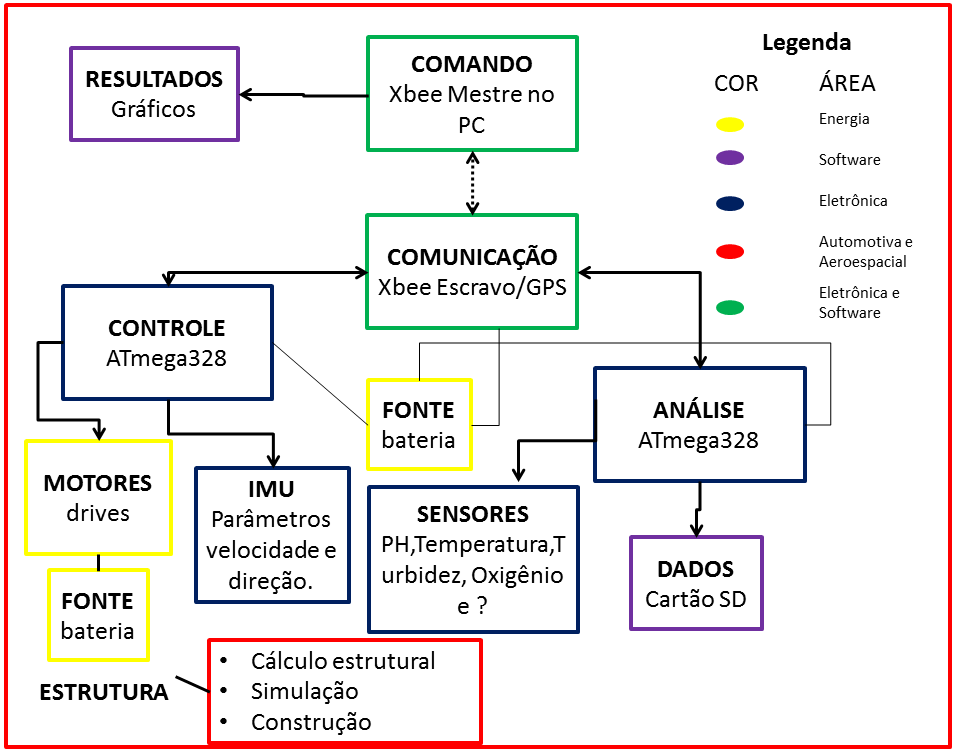
\includegraphics[scale=0.7]{figuras/diagramaGERAL}
	\caption{Diagrama de fluxo de sinais geral. Demonstra o funcionamento geral e como os componentes serão conectados. Assim podemos desmembrar o problema em tarefas mais simples.}
	\label{fluxodesinais}
\end{figure}


\FloatBarrier

\section{Subgrupo Comunicação}

\begin{figure} [!htp]
	\centering
	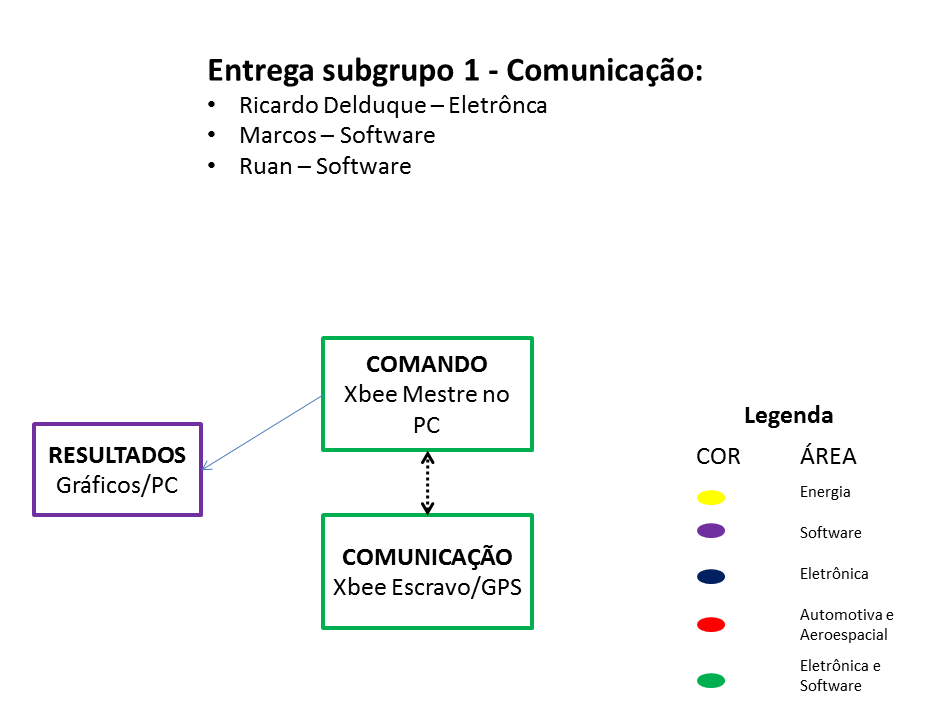
\includegraphics[scale=0.6]{figuras/subgrupocomuncacao}
	\caption{Relaciona os membros e os problemas e os componentes que o subgrupo irá trabalhar na área de comunicação de dados.}
	\label{subgrupocomunicacao}
\end{figure}
\FloatBarrier
Xbee

Para controlar e receber os dados a distância escolhemos a tecnologia da Xbee Fig. \ref{Xbee} por sua compatibilidade com \textit{standalone} personalizado "RoBoatino" (nossa versão do Arduino) e alcance de até 1,5 km de distância em área externa. Usaremos uma mestre conectada a um computador e uma escrava dentro do RoBoat.
 \begin{figure} [!htp]
	\centering
	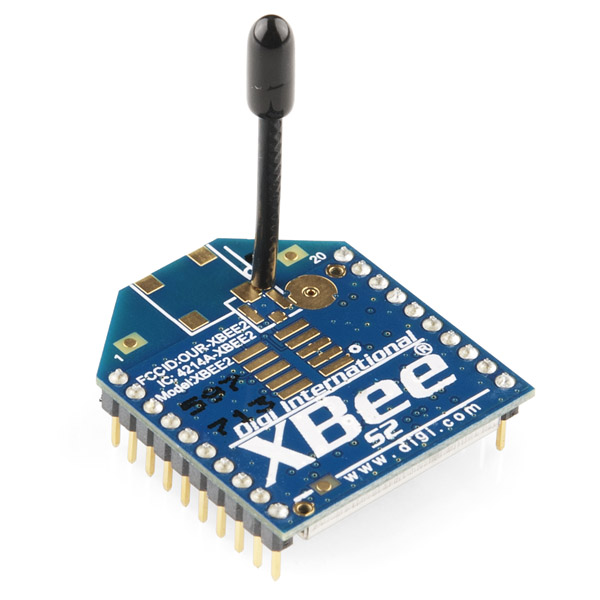
\includegraphics[scale=0.5]{figuras/Xbee}
	\caption{Modulo Xbee pro serie 2 com antena.}
	\label{Xbee}
\end{figure}
\FloatBarrier
Este módulo XBee PRO da Série 2 é um formato físico de uma família de modems de RF fabricado pela Digi International (MaxStream®) que utiliza o padrão ZigBee IEEE 802.15.4. A Série 2 possui uma melhora no que diz respeito a potência de saída e protocolo de dados, permitindo uma comunicação de forma simples entre microcontroladores, computadores, sistemas, ou qualquer periférico que utilize porta serial.



A ZigBee Alliane junto ao IEEE (Institute of Electrical and Eletronics Engineers) trabalham em conjunto para proporcionar e desenvolver tecnologias para criar um padrão de baixo consumo de energia, baixo custo, segurança, confiabilidade, e com funcionamento em rede sem fios (wireless) baseado em uma norma aberta e global.



Os módulos RF padrão ZigBee operam na freqüência ISM (Industrial, Scientific and Medical), sendo na Europa de 868 MHz (1 canal), 915 MHz (10 canais) nos Estados Unidos e 2,4 GHz (16 canais) em outras partes do mundo, e não requerem licença para funcionamento. Eles foram criados para economizar o máximo de energia e se comunicarem uns com os outros na forma e roteamento de sinais de forma similar as abelhas que voam aparentemente em Zig-Zag, daí o nome ZigBee, e dessa forma, durante um vôo a trabalho as abelhas em busca de néctar trocam informações com outros membros da colmeia sobre distância, direção e localização de onde encontrar pólen. Este modo de configuração de rede permite a dispositivos com ZigBee encontrarem outros dispositivos de forma apropriada, automática e configurar vários caminhos possíveis entre cada nó da rede para a passagem da informação, pois já que numa única rede podem existir mais de 65 mil nós ZibBee então a rede pode ser distribuída por centenas ou milhares de quilômetros quadrados sem prejuízo de comunicação. E se algum nó falhar, uma rota alternativa é automaticamente encontrada, simplesmente mudando o percurso da informação.



As Redes ZigBee oferecem uma excelente imunidade contra interferências, sendo ideal para aplicações industriais, mesmo em ambiente hostil e de fortes ruídos, pois mantem a integridade da comunicação. Também pode ser destinado ao uso residencial, pois possui longo alcance e baixíssimo consumo.


Características:
Performance
- Rendimento da Potência de saída: 63 mW (+18 dBm) / 10 mW (+10 dBm) EIRP;
- Alcance em ambientes internos/zonas urbanas: 90m;
- Alcance de RF em linha visível para ambientes externos: 1,5Km;
- Sensibilidade do receptor: -102 dBm (1\% PER);
- Freqüência de operação: 2,4 GHz;
- Taxa de dados de RF: 250 Kbps;
- Taxa de dados serial (Data Rate): 1.200 bps a 1Mbps;
Alimentação
- Tensão de alimentação: 2,7 à 3,6V;
- Corrente de transmissão (típico): 205 mA em 3,3 V;
- Corrente de Recepção (típico): 47 mA em 3,3 V;
- Corrente de Repouso: 3,5 microA em 25ºC;
Propriedades físicas
- Dimensões: (2,438cm x 3,294cm);
- Peso: 3,5g;
- Temperatura de operação: -40 a +85ºC (industrial);
- Antena integrada no módulo do tipo: Arame (wire whip);
Rede
- Tipo de espalhamento espectral: DSSS (Direct Sequence Spread Spectrum);
- Manipulação de erro: Retransmite novamente (Retries) e reconhecimento (acknowledgements);
- Topologia de Rede: Peer-to-peer (Par-a-par), ponto-a-ponto, ponto-a-multiponto e malha;
- Endereçamento: 65.000 endereços de rede disponíveis para cada canal;
- Opções de filtros: PAN ID, canais e endereços;
- Criptografia: 128-bit AES;
- Número de canais selecionáveis via software: 14 canais de seqüência direta;
Geral
- Faixa de freqüência: 2,4000 - 2,4835 GHz;
- 06 pinos de entrada com ADC 10-bit;
- 08 pinos de entrada/saídas.

Iremos estudar o funcionamento da Xbee através de cinco aula de um professor americano disponibilizadas no Youtube. XBee Basics - Lesson 1 até 5. Usando o guia da figura \ref{xbeeguide}

 \begin{figure} [!htp]
	\centering
	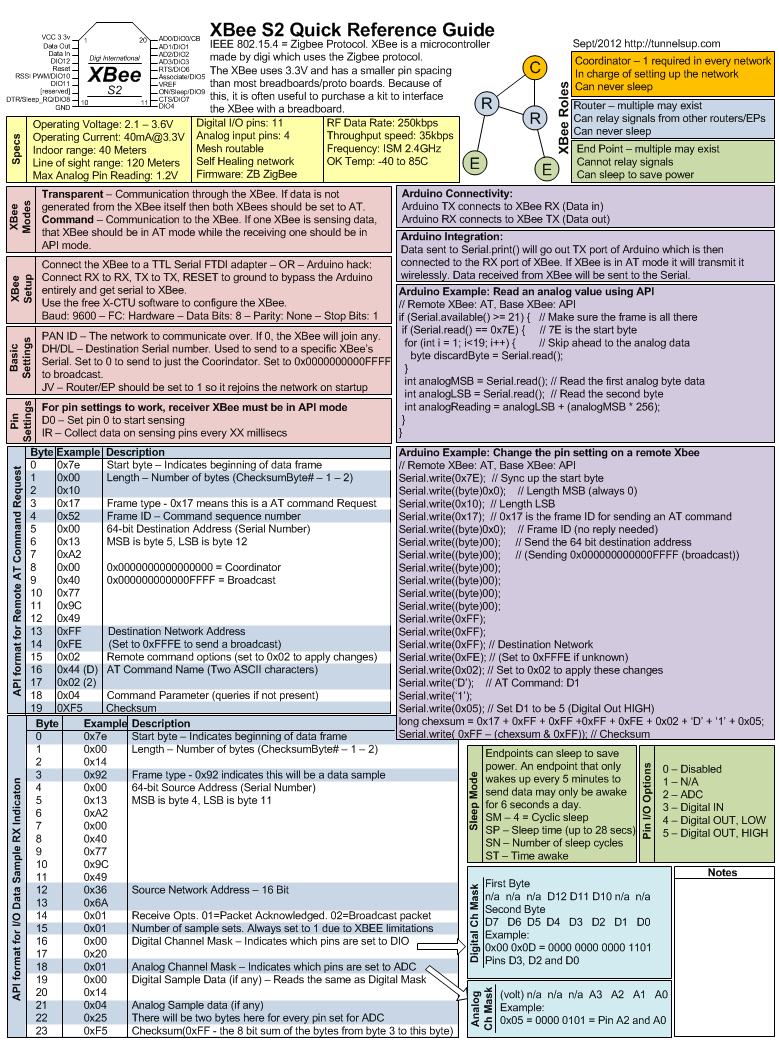
\includegraphics[scale=0.6]{figuras/xbeeguide}
	\caption{Guia de estudos para trabalhar com Xbee. Um resumo com todas as informações relevantes.}
	\label{xbeeguide}
\end{figure}
\FloatBarrier

GPS

O Módulo GPS é um dispositivo eletrônico especialmente desenvolvido para aplicação em projetos robóticos ou domóticos que tenham como base plataformas de prototipagem, entre elas, o Arduino, o Raspberry PI, etc.
- O Módulo GPS funciona em conjunto com a plataforma microntroladora, informando ao Arduino, se for o caso, a localização exata de determinado objeto em que o Módulo GPS esteja instalado, enviando dados referentes a latitude e longitude, data, hora e velocidade de deslocamento.
- A instalação do Módulo GPS junto ao Arduino, na grande maioria dos projetos, dá-se em protótipos aéreos, onde o usuário pode controlar via smartphone ou computador as coordenadas e a velocidade do objeto prototipado.
- Outra importante aplicação que pode ser dada ao Módulo GPS é comandar um robô para executar diferentes tarefas em localizações e horários predefinidos.
- Para executar tais tarefas o Arduino ou o Raspberry PI precisam ser programados, e pode ser necessário a aplicação de outros acessórios.
- Uma informação importante do Módulo GPS é sua interface serial de 3,3V, não tolerando 5V. Deste modo, se o microcontrolador tiver um GPIO de 5V, será necessário o uso de um level shift.
- Não deixe de adquirir o Módulo GPS para Arduino e Raspberry PI e entregue mais funções e comodidade aos seus projetos, seja ele aéreo ou terrestre
COMO FUNCIONAM OS MÓDULOS GPS

Atualmente é indiscutível a importância de sistemas de posicionamento por satélites em equipamentos como sistemas de navegação de automóveis, navegação aérea e marítima, cartografia, meio ambiente, agricultura etc.

Também muitos profissionais da área e robistas desejam criar seus projetos que utilizem um módulo GPS, desses comprados em lojas de robótica, e conectar à um microcontrolador, como o PIC ou uma placa arduíno.

Neste artigo, pretendo mostrar de forma breve o princípio de funcionamento dos módulos GPS e como os dados são recebidos e interpretados. Em seguida vou compartilhar como identificar a latitude e a longitude de um módulo GPS modelo ATK-NEO-6M-V23 através de um microcontrolador PIC e mostrar esses dados em um display LCD.
    
Funcionamento básico

O sistema GPS consiste de 24 satélites na órbita terrestre a uma altitude de 20.000 Km. Eles fazem a trajetória completa ao redor da terra em cerca de 12 horas. Para localizar e calcular a posição de um módulo receptor de GPS são necessários pelo menos 3 satélites. Com um quarto satélite é possível determinar a altitude do receptor. 

Padrão de formato de dados NMEA

O padrão utilizado para a comunicação GPS é o NMEA 0183 (National Marine Electronics Association). É utilizado pela marinha americana e define os requisitos elétricos de sinalização,  protocolo de tempo e de comunicação de dados.

O módulo GPS recebe os dados em uma sequência de caracteres no formato ASCII. Essa sequência é chamada de sentença e é formada por caracteres sequenciais, separados por vírgulas (",") que definem a latitude, longitude, data e hora além de outras informações sobre a posição do satélite.
 Sentença RMC

Existem vários tipos de sentenças recebidas por um módulo GPS (RMC, GGA, GSA entre outras), porém neste caso iremos tratar da sentença RMC (Informação mínima de navegação recomendada - tipo C).O padrão RMC tem a seguinte sequência:
\begin{itemize}

\item A sentença sempre inicia com o caractere “\$” ;
\item Após esse caractere, são recebidos frases pré-definidas com campos separados por “,” (vírgulas);
\item O caractere “*” (asterisco) sinaliza que os próximos dois caracteres são referentes ao checksum;
\item O checksum são 2 caracteres que servem para verificar a integridade dos caracteres recebidos;
\item Após os caracteres de checksum são recebidos ainda os códigos ASCII do <LF> (line feed) e <CR> (carriage return).
\end{itemize}

\section{Subgrupo Controle de motores}

\begin{figure} [!htp]
	\centering
	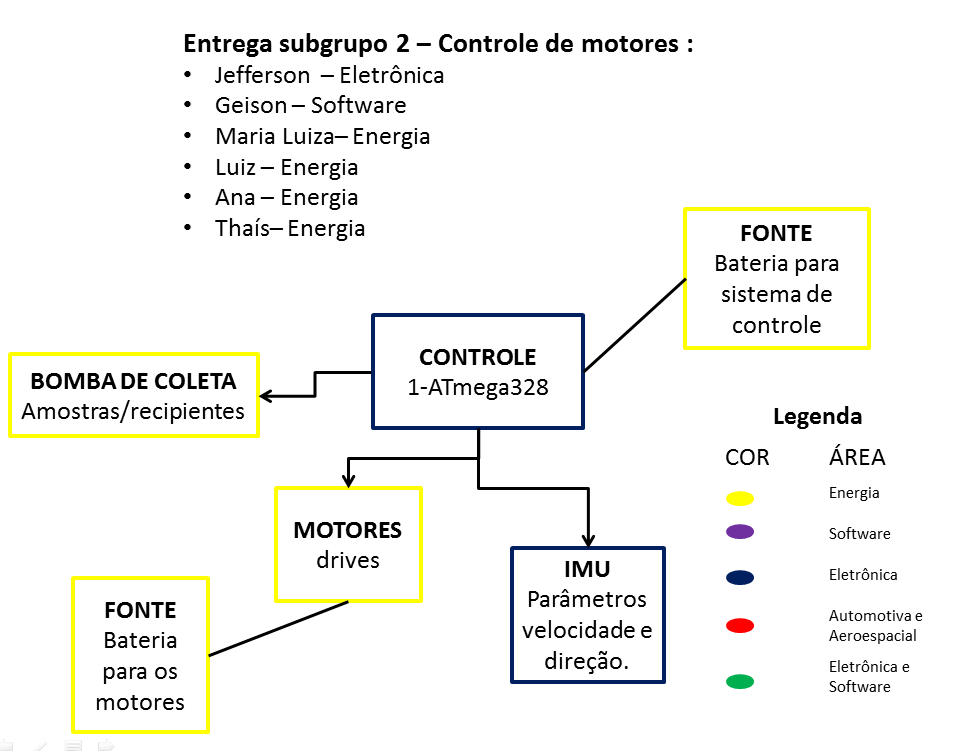
\includegraphics[scale=0.6]{figuras/subgrupocontroledosmotores}
	\caption{Relaciona os membros e os problemas e os componentes que o subgrupo irá trabalhar na área de controle dos motores.}
	\label{subgrupocontroledosmotores}
\end{figure}
\FloatBarrier
ATmega328
              
Microcontrolador Atmel ATmega328

O microcontrolador ATmega328 da Atmel é utilizado nos Arduinos mais recentes. É um microcontrolador de 8 bits, com arquitetura Harvard modificada. Um Pouco Sobre a Família AVR

O ATmega328 pertence à família AVR da Atmel. Todos os modelos desta família compartilham uma arquitetura e conjunto de instruções básicas, particularmente os grupos tinyAVR (microcontroladores ATtiny), megAVR (os ATmega) e XMEGA (os Atxmega).Os primeiros modelos de Arduino usavam o ATmega8 (com 8K de memória Flash), que posteriormente foi substituído pelo ATMega168 (com 16K de Flash e maiores recursos de entrada e saída) e finalmente pelo ATMega328 (com 32K de Flash). A versão DIP destes três modelos compartilham a mesma pinagem (porém o ATMega168 e ATMega328 permitem alguns usos diferentes dos pinos). O Arduino Mega 2560 usa o ATMega2560 com 256K de Flash e uma capacidade muito maior de entrada e saída.




 \FloatBarrier
 \begin{figure} [!htp]
	\centering
	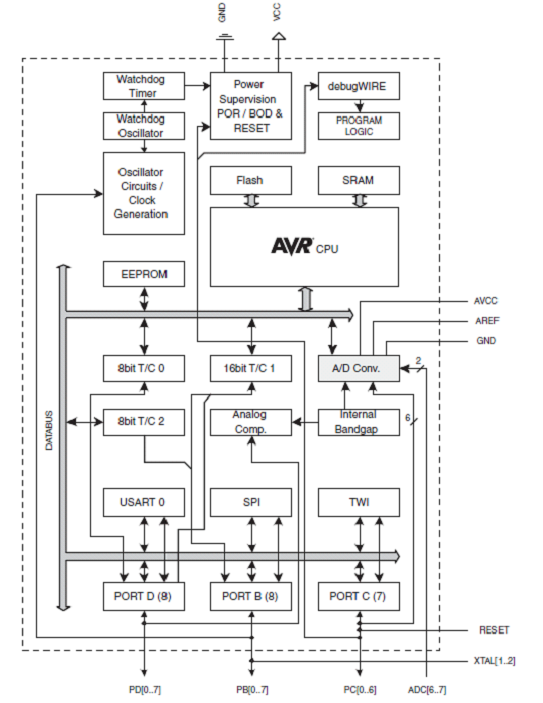
\includegraphics[scale=0.6]{figuras/atmega328}
	\caption{O Diagrama de Blocos, extraída do datasheet, mostra os principais blocos do microcontrolador.}
	\label{atmega328}
\end{figure}
\FloatBarrier

Reparar as ligações separadas entre a CPU e as memórias Flash e SRam. O uso de vias de dados separadas para programa e dados é uma característica da arquitetura Harvard. Na família AVR as duas vias tem largura de 8 bits e a memória Flash pode ser usada para armazenar dados constantes (daí ser uma arquitetura Harvard modificada). 

Entretanto, somente instruções armazenadas na Flash podem ser executadas (não é possível executar código que esteja na SRam).
Como outros microcontroladores AVR, o ATMega328 possui ainda uma memória do tipo EEProm, porém esta memória está ligada na via de conexão aos periféricos e portanto não é acessada pelas instruções normais de acesso a memória.

Além da EEProm podem ser vistos as três portas de E/S digital (PORTs B, C e D), os três timers (TCx, dois de 8 bits e um de 16 bits), o conversor A/D, o comparador analógico e as interfaces seriais SPI, TWI (compatível com I2C) e USART. 


CPU

A Arquitetura Interna da CPU:

\FloatBarrier
 \begin{figure} [!htp]
	\centering
	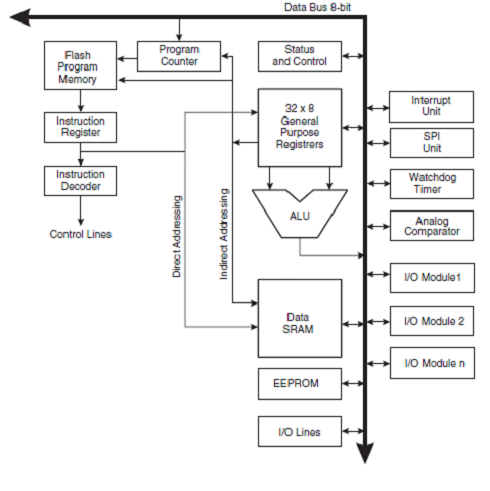
\includegraphics[scale=0.6]{figuras/cpuatmega}
	\caption{O coração de um microcontrolador é a sua CPU. No caso do ATmega328, temos uma CPU AVR do tipo “enhanced core“. Vejamos algumas de suas características..}
	\label{cpu}
\end{figure}
\FloatBarrier

Novamente notamos a separação das vias de acesso à Flash e SRam, típicas das arquiteturas Harvard e derivadas.
No lado da Flash temos o Program Counter (que aponta para a próxima instrução). O AVR possui um pipelinede um nível, no qual enquanto uma instrução é executada a seguinte é carregada. Isto possibilita executar as instruções mais simples em um único ciclo de clock. Embora a Flash seja endereçada byte a byte, as instruções são compostas por uma ou duas palavras de 16 bits (ocupando portando duas ou quatro posições da Flash).
A família AVR possui uma generosa coleção de 32 registradores de uso geral, todos de 8 bits. Os seis últimos registradores podem ser usados aos pares como três registradores de 16 bits (X, Y e Z) para endereçamento indireto da memória.
A Unidade Lógica Aritmética (ALU) trabalha com 8 bits; obtêm os operandos dos registradores e coloca o resultado no primeiro operando (exceto na multiplicação). Todas as operações lógicas e aritméticas são executadas em um ciclo, exceto pela multiplicação que demora dois ciclos.


Memória Interna de Dados

A memória interna de dados é composta pelos registradores de uso geral, os registradores de entrada e saída (que controlam os periféricos internos) e a memória SRam propriamente dita.
No Atmega328 os registradores podem ser acessados nas primeiras 32 posições de memória e os registradores de E/S nas 64 posições seguintes, com a SRam começando no endereço 0x60.
Reparar que na figura não temos a pilha nem o seu ponteiro (SP). No AVR a pilha reside na memória SRam e o seu ponteiro são dois registradores de E/S.


Como todo microcontrolador que se preze, o ATmega328 possui uma boa coleção de periféricos internos. A plataforma Arduino se aproveita disto e disponibiliza quase todos os pinos do ATmega para os shields, como mostram as figuras abaixo


\FloatBarrier
 \begin{figure} [!htp]
	\centering
	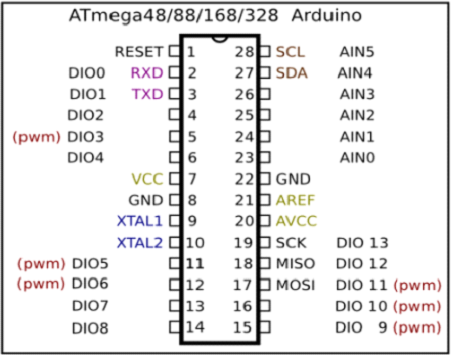
\includegraphics[scale=0.6]{figuras/pinagematmega}
	\caption{Podemos ver a relação dos pinos para o circuito integrado Atmega328.}
	\label{pinagematmega}
\end{figure}
\FloatBarrier

IMU

A Unidade de Medida Inercial (IMU) é um dispositivo eletrônico que mede e relata a força específica do corpo, velocidade angular e o campo magnético em torno do corpo, usando uma combinação de giroscópios acelerômetros e barômetros.Um IMU permite que um receptor GPS para trabalhar quando de GPS sinais não estão disponíveis, como em túneis, no interior de edifícios, ou quando a interferência eletrônica está presente.

 \begin{figure} [!htp]
	\centering
	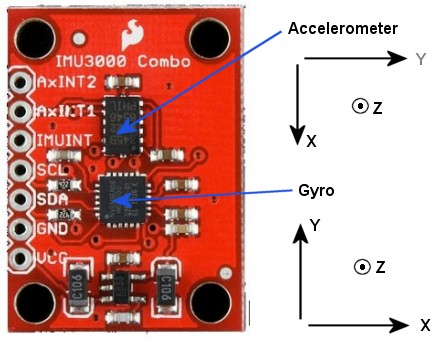
\includegraphics[scale=0.6]{figuras/IMU}
	\caption{Módulo de uma unidade lógica inercial compatível com arduino.}
	\label{IMU}
\end{figure}
\FloatBarrier


Sistema propulsivo 


Para obtenção das características necessárias para a escolha do motor, será necessária que haja a estimativa de alguns valores, a fim de se obter informações suficientes para poder realizar posteres cálculos.


Estimativa:O cálculo da potência de eixo do motor depende da resistência ao avanço que o barco possui. A resistência ao avanço é uma função dependente do número de Reynolds e do número de Froude. Para tal, a seguir é calculado tais números adimensionais:
\begin{equation}\label{Reynolds}
Reynolds = \frac{V * Lf}{v} 
\end{equation}
Substituindo V por 1,38 m/s, Lf por 0,60 m e v por 0,000001007 $m^2$/s; encontramos 8,22 * $10^5$ .

 
O número de Reynolds é maior que 2100, logo temos escoamento turbulento.É importante mencionar que para o cálculo de Reynolds, foi inicialmente fixado uma velocidade de 5 $km/h$.Que é a velocidade fixa que o barco irá se locomover.

\begin{equation}\label{Froude}
	Froude = \frac{V}{\sqrt{g * Lf} }
\end{equation}

Substituindo V por 1,38 m/s, g por 9,81 m/$s^2$ e Lf por  0,60 m; encontramos 0,568.

O número de Froude é menor que 1, logo temos escoamento fluvial
Sendo, 
Lf = Comprimento de linha de flutuação
V = velocidade de avanço do barco
v = viscosidade cinemática da água à 20ºC
g = gravidade
 
Equações dos coeficientes relacionados a propulsão

Velocidade de avanço:Cb é o coeficiente adimensional de finura total. Dado por, segundo o método de Van Lameren equação \ref{Cb}:

\begin{equation}\label{Cb}
	Cb  = \frac{1,37 - (2,02 * V)}{\sqrt{Lf} }
\end{equation}
 Substituindo a equação \ref{Cb} temos: Cb= $1,37 - (2,02 * 1,38)/\sqrt{1,10}  $
 
Sendo, 
Lf = Comprimento de linha de flutuação
V = Velocidade de avanço do barco

$\omega$ é o coeficiente adimensional de esteira. Dado por, segundo o método de Taylor:

$\omega$ = -0,05 + 0,50 * Cb  = -0,05 + 0,50 * 1,3516 = 0,6258


$\omega$ = V * Va / V 

Sendo, 
$\omega$ = Coeficiente de esteira

V = velocidade de avanço do barco

Va = velocidade com a qual a agua flui para o propulsor

Método de Schronherr  

Cálculo de Potência do motor:A potência do motor é calculada é calculada através da seguinte equação \ref{Schronherr}, onde é relacionada a resistência que o barco enfrenta e a velocidade que se deseja atingir.

\begin{equation} \label{Schronherr}
	Pe=Rt*Vs
\end{equation}
 

Onde,
Pe é e a potência efetiva, 
Rt a resistência total 
Vs a velocidade de serviço.

A resistência total é dada pela equação \ref{Rt}. 

\begin{equation} \label{Rt}
   Rt=Rw+Rv+Rb+Ra+Rf
\end{equation}
 

Onde,
Rw= Resistência da onda, desconsiderada no presente trabalho.
Rv= Resistência de viscosidade.;
Rb= resistência do bulbo, desconsiderada no presente trabalho, já que o barco não possui bulbo;
Ra= Resistência de arrasto.
Rf = Resistência Friccional

Coeficiente de forma.

Determina uma relação com o arrasto de uma placa plana com o do casco do barco. Utilizando o método de Holtrop e Mennen, temos que o fator de forma é calculado seguindo a expressão: 


\begin{equation}\label{k1}

    1+k1=0,93+(TL)^{0,2283}  * (BLr)^{0,92497}  * (0,95+Cp)^{-521448}  *(-1+Cp-0,0225)^{0,6906} 
\end{equation}


Os valores da Boca, calado e áreas frontal e total são apresentados na tabela abaixo:


\begin{table}[h]
	\centering
	\label{casco}	
	\begin{tabular}{cc}
		\toprule
		\textbf{Parâmetro} & \textbf{Dimensão}  \\
		\midrule
		S total  & 0,84 (m$^{2}$)       \\
		S frontal  & 0,18 (m$^{2}$)          \\
		B  & 0,6 (m)               \\
		T  & 0,05 (m)   \\
		\bottomrule
	\end{tabular}	
	\caption{Características do casco}
\end{table}

Onde, 

Cp adimensional é dado pela razão entre o  volume do casco e a área transversal vezes o comprimento L eq. \ref{Cp},

\begin{equation} \label{Cp}
    Cp = \frac{Volume}{ S * L}
\end{equation}

    $Cp = \frac{0,336 m^{3}}{ 0,84 m^{2} * 1,10 m}$
    
    Cp = 0,363
    
O comprimento do corpo de ré, Lr pode ser calculado pela seguinte expressão, utilizando novamente o método de Holtrop e Mennen.

\begin{equation} \label{Lr}
    Lr = \frac{1 - Cp + (0,06 * Cp)}{4Cp - 1} 
\end{equation}

   $Lr = \frac{1 -0,363 + (0,06*0,363)}{(4*0,363) - 1} $
   
   Lr = 1,45 m

O cálculo do fator de forma:


 1+k1=0,93+(\frac{0,05}{1,10})$^{0,2283}$  * (\frac{0,6}{1,45})$^{0,92497}$  * (0,95+0,363)$^{-521448}$  *(-1+0,363-0,0225)$^{0,6906}$

1 +k1= 0,93 + (0,493 * 0,442 * 1,32 * 0,750)

1 +k1  = 1,146

Resistencia de viscosidade

A equação é dada por:

\begin{equation} \label{Rv}
   Rv = 0,5pv^2 * Cf(1+k)*Stotal
\end{equation}
 

Onde, 

$\rho$ = massa especifica da água;

v= velocidade de serviço;

Cf= Coeficiente de placa plana, dado pela eq. \ref{Cf}

(1+K)= Coeficiente de formadado pela eq. \ref{k1}

Sm = Area total molhada.


\begin{equation} \label{Cf}
	Cf=\frac{0,075}{(log Re-2)^2}
\end{equation}



$Cf = \frac{0,075}{(log 8,22 * 10^{5}-2)^{2}}$

$Cf = \frac{0,075}{(5,914 * 10^{5}-2)^{2}}$

$Cf = \frac{0,075}{(15,32}$

$Cf = 4,89 * 10^{-3 }  $\\


A resistência de viscosidade pode então ser calculada:  
  
$Rv=0,5 * 1000 (kg/m^{3}) * 1,942(m/s)* 4,89 * 10^{-3} * (1,146) * 0,51 (m^{2})$

Rv = 5,37 N\\

Onde, 

$\rho$ = massa especifica da agua;

V = velocidade de serviço;

Cf = Coeficiente de arrasto de placa plana, dado pela eq. \ref{Cf}

(1+K) = Coeficiente de forma, dado pela eq. \ref{k1}

Sm = Area total molhada.\\
   
Resistência friccional.

A equação é dada por:

$Rf = 0,5 v^{2} * Cf * Sm$

Com todos os dados, podemos calcular a resistência friccional:
  
$Rf=0,5 * 1000 (kg/m^{3}) * 1,942* 4,89 * 10^{-3} * 0,51 (m^{2})$

Rf= 4,69 N  \\


Resistência de arrasto:A resistência de arrasto a ser considerada consiste na resistência que o fluido ar aplica ao barco. Ela é dependente da velocidade que o barco possui, da área de referência e do coeficiente de arrasto dependente da forma do barco.

A resistência de arrasto é dada pela fórmula a seguir:

$Ra = 0,5 x \rho x V^{2} x Ca A$

Onde, 

$\rho$ = massa especifica do ar à 20ºC;

V = velocidade de serviço;

Ca = Coeficiente de arrasto

A = Area de ação (frontal)

De acordo com Çengel e Cimbala, 2015, o coeficiente de arrasto  para uma haste triangular, no qual se aproxima ao formato da popa do barco, é de 1,5.

$Ra = 0,5 * 1,2041 * 1,94^{2} * 1,5 * 0,18$

Ra = 0,612 N 

Resistência Total e Potência do Motor

$Rt=Rv+Ra + Rf = 5,37 + 4,69 + 0,612$

Rt = 10,672 N

Assim podemos calcular a potência efetiva estimada

Pe=Rt*V

Pe = 10,672 N x 1,94 m/s 

Pe = 20,70 W

Pe = 0,028 cv

\\

Eficiência

Segundo Guesse, 2016, a eficiência dos propulsores variam de 55\% à 58\%. O INMETRO determina que a eficiência de motores elétricos com menos de 0,75 cv seja superior à 80\%.

d= Eficiencia propulsiva estimada de 55\%

s=Eficiência do sistema motorestimada em 80\%

Eficiência total (t) = 0,80 x 0,55= 0,44 = 44\%


Margens de Segurança

Considerando uma margem de segurança de 10\%.

Potencia Real

O cálculo da potência, tendo em consideração a eficiência estimada do sistema motor, eixo e propulsor:

Potencia Real = 20,70W

0,44= 47,05 x 1,10 

= 51,75W 

= 0,070cv.


Cálculo do torque do motor

As forças de torque e potência são energias que aparecem a partir do momento em que o barco começa a se movimentar. Dos dois, o torque é o responsável pela capacidade do motor produzir força motriz, ou seja, o movimento giratório. É essa força que faz o barco sair da inércia e se movimentar. Para o cálculo do torque utiliza-se a seguinte equação:
    
    $\tau$ = d*F
    
Onde :

$\tau$ = torque

d =distancia dos eixos

F = força


 $\tau$   = 0,15 x 10,672 = 1,60 N.m

Escolha do Motor

Feito o cálculo da potência real e do Torque podemos fazer a escolha dos motores. Utilizaremos dois motores de corrente contínua modelo F 006 B20 103, pesando aproximadamente 1Kg. O custo estimado de cada motor é de 235 reais. 


\FloatBarrier
\begin{figure} [!htp]
	\centering
	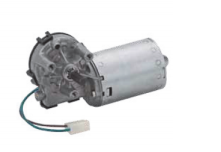
\includegraphics[scale=0.6]{figuras/motor2}
	\caption{Modelo dos motores utilizados.}
	\label{motor2}
\end{figure}
\FloatBarrier

\FloatBarrier
\begin{figure} [!htp]
	\centering
	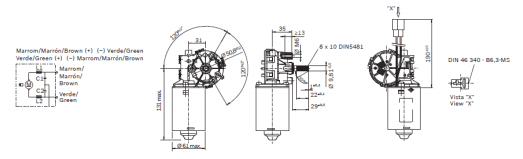
\includegraphics[scale=0.6]{figuras/cotas}
	\caption{ Desenho técnico do motor, Fonte:Casa Ferreira
}
	\label{cotas}
\end{figure}
\FloatBarrier


\begin{figure} [!htp]
	\centering
	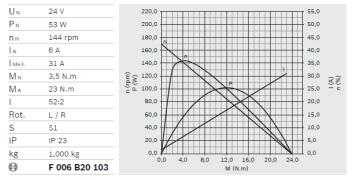
\includegraphics[scale=0.6]{figuras/especificacoes}
	\caption{ Especificações do motor}
	\label{especificacoes}
\end{figure}
\FloatBarrier

Definição das pás

A movimentação do veículo aquático de superficial irá ser gerada através de pás que estão ligadas ao motor por um eixo. O modelo do veículo de superfície aquática escolhido como base para o desenvolvimento deste projeto utiliza o mecanismo de rodas d’água. O seu princípio de funcionamento irá converter a energia existem em um fluxo de fluido em energia mecânica. O funcionamento dessas pás no projeto do Roboat acontecerá da seguinte forma, o motor irá acionar a roda através do eixo girante, transformando a energia elétrica em mecânica e o fluxo de água irá auxiliar no movimento do barco.

\FloatBarrier


\begin{figure} [!htp]
	\centering
	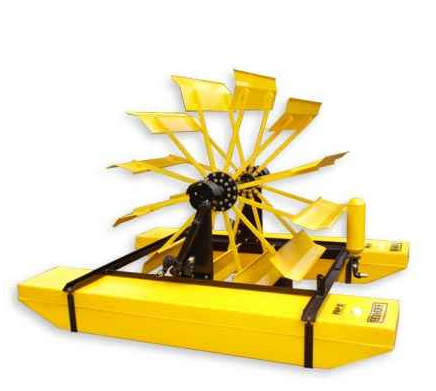
\includegraphics[scale=0.6]{figuras/pas}
	\caption{ Especificações do motor}
	\label{pas}
\end{figure}
\FloatBarrier

Como o projeto escolhido como referência para o Roboat não possui informações se faz necessário uma estimativa da dimensão da roda d’água.

Estimativa da dimensão da roda  

Para estimarmos o raio das rodas levaremos em conta o Torque do motor, com isso temos:

$\tau$motor= Fn * Rt

Fn= Força necessária

Sabemos que Fn>Rt, Para uma boa margem de segurança vamos assumir que Fn=2*Rt.
Como, 

Rt=10,672N 

Fn= 21,344

Com isso podemos calcular o raio das rodas, o torque nominal do motor utilizado é de 3,5N.m.
Assim,

$roda=\frac{3,5}{21,355}$
roda = 0,16m

Logo, nossa roda necessita de aproximadamente 32 cm de diâmetro.

Estimativa da dimensão das pás

Tendo o raio das rodas agora precisamos estimar as pás, para isso vamos calcular a área necessária para cada uma, esse calculo é dado pela equação a seguir:

$Apás=\frac{Fn}{P}$

onde, 
P= Pressão da água;

A Pressão pode ser calculada pela expressão a seguir:

$P=\frac{\rho*v^2}{2}$

onde v é a velocidade, logo a pressão é:

$P=\frac{1000*(1,38)^2}{2}$
P = 952,2 Pa

Calculando a área das pás

$Apás=\frac{21,344}{952,2}$
Apás = 0,022 metros quadrados 

Considerando uma pá retangular, temos:

Apás=l*sen(teta)*b

onde, 
l= altura das pás
b= base das pás 
teta= angulo de inclinação 

Para terminar o dimensionameto, estimamos valores para teta e para a base das pás. 

Teta= 90°
b=27cm

A partir desses valores achamos que altura das pás deve ser de 8 cm.

Estimativa do sistema de bombeamento
    
O sistema de bombeamento será utilizado para a coleta das amostras de água que serão armazenadas para futuras análises laboratoriais. Os parâmetros para análise não possuem um valor específico, ou seja, para cada parâmetro existe um volume de amostra. A maioria das análises precisam em torno de 100ml a 250ml. Por isso as coletas do Roboat será feita com uma capacidade de 250ml (NBR, 1987). Essa estimativa será adaptável a demanda do cliente, ou seja o volume de água a ser coletado deverá ser previamente acordado.

Calculo de dimensionamento:

As exigências da bomba são:

Vazão (Q) = $6x10^{-5} m^{3}/s$
    
Altura manométrica (H) = 0,5m
    
Numero de rotações (RPM) = 400
    

A velocidade específica é:

$ns = \frac{3,65 * n * Q^{0,5}}{H^{0,75}} $

$ns = \frac{3,65 *  400 * 0,00006}{0,5^{0,75}} $

 ns = 5,21 rpm.
 
 Como ns < 90 rpm trata-se de uma bomba centrifuga radial.

$nq = \frac{5,21}{3,65}$

$nq = 1,42 rpm$

Correção de descarga:

Considerando pressão baixa, pode-se considerar um fator de correção de 5\%

Q’ = Q + (0,05 x Q)

Q’= 0,00006 + (0,05 x 0,00006)

Q’= 0,000063 m$^{3}$/s


Potencia motriz:

Bombas centrifugas possuem rendimento entre 10\% e 85\%, como se trata de uma bomba de baixa vazão, consideramos eficiência como 10\%

$N = \frac{1000 *Q' * H}{75 * n}$

$N = \frac{1000 * 0,000063 * 0,52}{7,5 * 0,1}$
 
$N = 0,0115 cv$

Diâmetro de eixo:\\

    $de = 12 * (\frac{N}{n})^{1/3}$
    
    $de = 12 * (\frac{30,0115}{400})^{1/3}$
    
    $de= 0,030 cm$
    
Diâmetro de núcleo\\

    dn = de + [2 x (0,05cm)
    
    dn = 0,030 + (2 x 0,05)
    
    dn = 0,13cm
    
    dn = 0,0013m
    
Velocidade média na boca:\\

    Para nq < 10, Kr1 = 0,090
    
    V’1 = Kr1 x 2 x g x H
    
    = 0,090 x 2 x 9,81 x 0,5
    
    = 0,281 m/s
    
Diâmetro da boca de entrada do rotor:\\

$d1’ = 4 * Q' * V'1 + dn^{2} $

$d1’ = 0,017m$

$d1’ = 1,7cm$


Diâmetro médio da aresta de entrada:

dm1 = 1,05 x d1’ 
dm1 = 1,05 x 1,7
dm1 = 1,78cm

Velocidade meridiana de entrada:

Para nq<10, Kvm1 = 0,11

$Vm1 = Kvm1 x (2 * g * H)^{1/2}$

$Vm1 = Kvm1 x (2 * 9,81 * 0,5)^{1/2}$

$Vm1 = 0,344 m/s$

Velocidade periférica à entrada

$U1 =  \frac{\pi  x dm1 x n}{60}$

$U1 = \frac{\pi  x 0,0178 x 400}{ 60}$

$U1 = 0,372 m/s$


Angulo de entrada das pás:

$tg \beta1= \frac{Vm1}{U1}$

$tg \beta1= \frac{0,344}{ 0,372}$

$\beta1= 42,76º$


Numero de pás:

Segundo Macintyre, 1997, o cálculo das pás segue a equação:

Z = $\pi$ x d2’ x 100
Onde d2’ = 1,1 x d1’= 1,1 x 1,7 = 1,87 cm
Z = $\pi$ x 0,0205 x 100 = 5,87
Dessa forma o número máximo de pás é 6.

Velocidade periférica à saida

$U2 =  \frac{\pi  x dm2 x n}{60}$

$U2 =  \frac{\pi  x 0,0187 x 400}{60}$

$U2 = 0,391 m/s$

Angulo de saída das pás:

Segundo Macintyre, 1997, para bomba de até 6 pás, o angulo $\beta$2 deve estar entre 22,3º e 30º.

A bomba escolhida para coleta será uma de refrigeração da CPU de um carro, sem escovas e à prova d 'água , modelo Submersível ES9P, que fará a coleta da água a temperatura ambiente e pressão atmosférica. A bomba fornece uma vazão volumétrica de 250 L/h e uma carga líquida (H) 0,5m. Seu funcionamento é por corrente contínua(DC) e tensão de 12V.

Como será necessária a coleta de 250 ml o tempo de sucção será de aproximadamente 4 segundos. De acordo com o escopo do projeto serão necessárias a coleta de três amostras e para que não haja contaminação das amostragem serão usadas três bombas para cada recipiente.

\FloatBarrier
\begin{figure} [!htp]
	\centering
	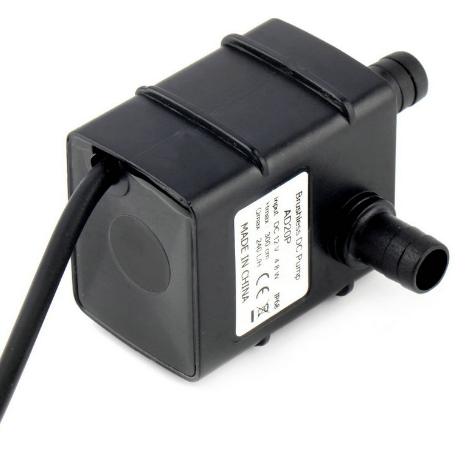
\includegraphics[scale=0.6]{figuras/bombaagua}
	\caption{Foto da bomba que colera água para nossas amostras.}
	\label{bombaagua}
\end{figure}
\FloatBarrier

Especificações:
\begin{itemize}
    \item Peso líquido 35g
    \item Dimensões  36 x 36 x 36 mm
    \item Corrente Nominal de 300mAh
    \item Preço R\$ 30,00
    \item Ruído < 45 dB
    \item Vida útil 30.000 horas
\end{itemize}


Baterias 

Para decidir a melhor bateria a ser utilizada é preciso saber quanto de corrente o sistema necessita. Nos nossos cálculos levaremos em conta só o necessário para suprir os motores, pois os componentes eletrônicos necessitam de pouco energia, podendo ser estimado.  

$I=\frac{P}{U}$

Onde, 

P é a potência do sistema (w)

U é a tensão (v)


Os dados de potência e tensão foram  obtidos através da Tabela \ref{especificacaomotor}.

$I=\frac{53}{24}$

$I=2,20 A$

Consideramos uma autonomia de 20 minutos.Então, para dois motores precisamos de aproximadamente 4Ah. Levando em consideração que os componentes eletrônicos e bombas iram precisar de energia da bateria e os valores e disponibilidades do mercado, usaremos duas baterias 12v 7ah, ligadas em série. O modelo das baterias esta apresentado na Figura \ref{bateria7}.

\FloatBarrier
\begin{figure} [!htp]
	\centering
	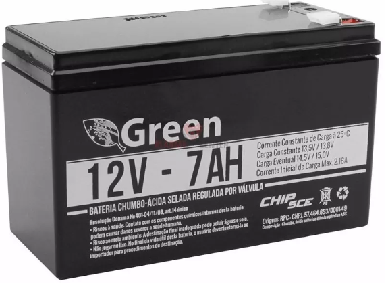
\includegraphics[scale=0.3]{figuras/bateria7}
	\caption{Foto da bateria}
	\label{bateria7}
\end{figure}
\FloatBarrier


Especificações:
\begin{itemize}
    \item Bateria Selada 12V VRLA (Estacionária);
    \item Tensão Nominal 12V;
    \item Capacidade Nominal 7 Ah;
    \item Peso médio 2 Kg;
    \item Tensão (V): 12;
    \item Dimensões Aproximadas: 9,5 x 6,5 x 15,1 cm;
    \item Preço: R\$ 57 cada.  
\end{itemize}


Modulo SD 


Os dados da análise de qualidade da água que forem coletados através dos sensores deverão ser armazenados no RoBoat, desta maneira se fez necessário um módulo SD que permita a utilização de um cartão de memória que receberá os dados que forem coletados pelos sensores, assim esses dados servirão de insumos para a elaboração dos gráficos relativos aos parâmetros da água. A vantagem é que caso haja perda de dados na transmissão sem fio poderemos recuperar os dados pela memória do cartão.

O Atmega 328 só possui 32kb de memória e pelo baixo custo de compra e implementação do cartão de memória a equipe optou por essa ação.

Este módulo permite a leitura e escrita em cartão SD (cartão de memória), com fácil ligação ao Arduino e outros microcontroladores. Todos os pinos de ligação estão identificados no módulo, que suporta formatos de arquivo FAT16 e FAT32, e alimentação de 3.3V ou 5V.

A comunicação é feita pela interface SPI (pinos MOSI, SCK, MISO e CS), e o nível de sinal é de 3.3V, exigindo um divisor de tensão para ligação à microcontroladores que trabalhem com 5V, como o Arduino.
\FloatBarrier
 \begin{figure} [!htp]
	\centering
	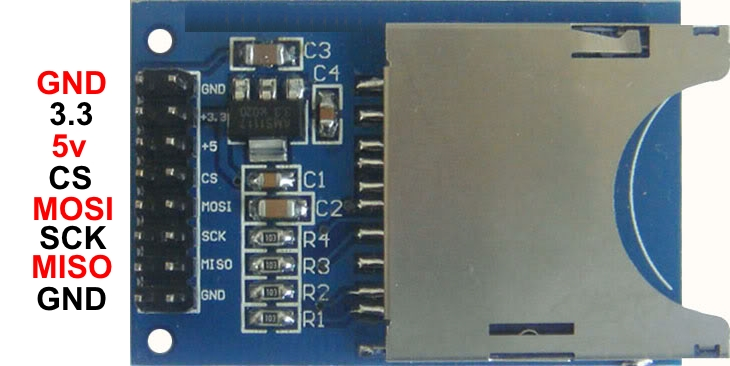
\includegraphics[scale=0.6]{figuras/cartaosdpinagem}
	\caption{Imagem ilustrativa do módulo de cartão de memória SD. Demonstra as funções de cada pino.}
	\label{cartaosdpinagem}
\end{figure}
\FloatBarrier

Sensor de Condutividade

A condutividade elétrica é a habilidade de um material permitir a passagem de corrente elétrica. A corrente elétrica flui na água através de íons. A quantidade de íons, o tipo dos íons e a temperatura do eletrólito influenciam na condutividade da água.
A condutividade da água também é um indicador de qualidade. A magnitude da condutividade propriamente dita não é importante, mas sim as variações abruptas que podem ocorrer durante um período de medição. A variação da condutividade na água significa que houve aumento significante de alguma substância. Um vazamento de esgoto, ou poluição por água residual agrícola irá aumentar a condutividade da água por possuir elementos como nitrato, fosfato e cloreto. Poluição causada por óleo ou qualquer matéria orgânica diminuirá a condutividade da água por serem elementos que não se dividem em íons.
Este sensor consiste em duas pontas de prova metálicas submersas numa solução aquosa. O princípio de medição deriva da lei de Ohm, em que a tensão aplicada nos terminais de um condutor é proporcional à corrente elétrica que o percorre. Para medir a condutividade da água é importante levar em consideração o efeito de polarização, eletrólise e a capacitância gerada oriunda das duas pontas metálicas em um meio dielétrico. Para evitar, ou diminuir, estes efeitos, deve ser utilizado um sinal de corrente alternada com frequência elevada. Por conseguinte, os íons não irão conseguir se depositar nas pontas metálicas e tampouco criar uma região polarizada. Assim, o sensor consistirá de três blocos principais. 

\begin{itemize}
	\item Oscilador
	\item Amplificador
	\item Conversor A/D
\end{itemize}

O circuito oscilador Ponte de Wien é um oscilador simples capaz de gerar ondas sinusoidais por meio de um amplificador operacional com realimentação positiva.

\FloatBarrier
 \begin{figure} [!htp]
	\centering
	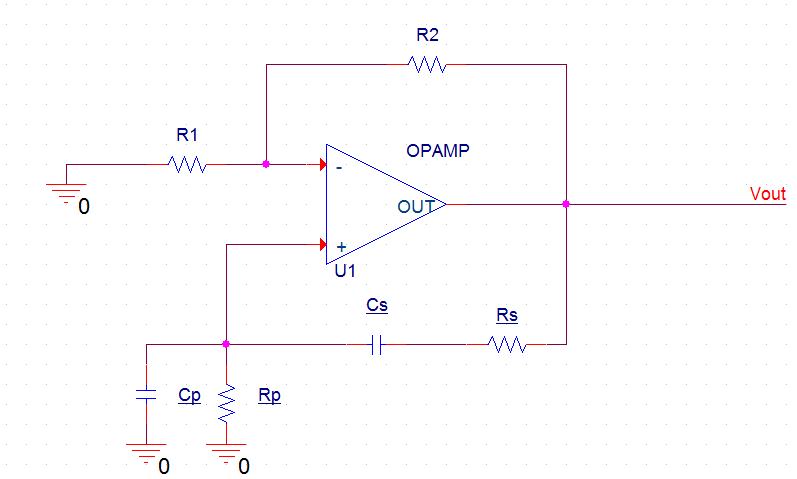
\includegraphics[scale=0.6]{figuras/pontewien}
	\caption{Circuito oscilador Ponte de Wien}
	\label{pontewien}
\end{figure}
\FloatBarrier

O bloco amplificador será utilizado para obter valores significativos de tensão que possam ser, posteriormente convertidos em um sinal de corrente contínua para, em seguida, ser traduzido em informação útil e, por final, transmitido. Este sensor, por sua simplicidade, também será desenvolvido pela equipe.
Os desafios são os mesmos comparado ao sensor de turbidez. A dificuldade e riscos estarão presentes na confecção da ponta de prova e também na calibração do dispositivo.


Sensor de turbidez
 
Turbidez é a medição da quantidade de luz dispersada pela interação de luz incidente com matéria suspensa não dissolvida em uma amostra de água. A turbidez pode ser interpretada como a medida da transparência da água e geralmente indica a presença de sólidos suspensos como limo, argila, silicatos, algas, matéria orgânica ou inorgânica, e até mesmo a presença de microrganismos. Estes sólidos suspensos contribuem para a cultura de microrganismos patogênicos por fornece-los abrigo e alimento. Além disso, dificultam o tratamento da água para sistemas de distribuição, quando por exemplo, há grande quantidade de matéria orgânica, aumentando a demanda por cloro. Estes patogênicos, caso não tratados corretamente, podem causar problemas gastrointestinais oriundos de água de má qualidade. Para ecossistemas aquáticos, a turbidez confere um aspecto importante aos organismos fotossintetizantes aumentando ou diminuindo sua concentração em determinadas áreas e, assim, afetando, por exemplo, a cadeia alimentar local. A importância da monitoração da turbidez se estende da qualificação de água potável a sistemas aquáticos naturais.

A unidade de medida da turbidez é a Unidade Nefelometrica de Turbidez (UNT), ou simplesmente, Unidade de Turbidez (uT). Esta, quantifica a magnitude de matéria suspensa na água por meio da medição da quantidade luz dispersada. Existem parâmetros que classificam a qualidade da água quanto a sua turbidez. De acordo com a portaria nº 2914/2011 do Ministério da Saúde, relativa a água tratada, o limite de turbidez para água subterrânea com desinfecção é de 5,0 uT, para água filtrada por filtração rápida é 0,5 uT e para agua filtrada por filtração lenta é 1,0 uT. Enquanto a resolução 357/2005 do Conselho Nacional do Meio Ambiente (CONAMA), relativa a águas superficiais brutas, na seção de água doce, estabelece para o padrão de qualidade da água o limite de 40 uT.

Os métodos existentes para medir a transparência da água muitas vezes exigem interferência humana, tais como vela de Jackson e tubo de Secchi, que consistem em analisar a transparência da água via visualização. Estes métodos estão descartados por demandar interferência humana, baixa precisão para pequenos volumes de água, e por impossibilitar a medição de forma remota. Para cumprir com os requisitos do projeto, a medição deve ser feita remotamente, deve ser precisa e realizada em tempo real, necessitando uma abordagem mais moderna. Existem três possíveis abordagens para medir a turbidez da água, todas usando emissores e receptores de luz em que seus resultados dependem da quantidade de sólidos suspensos, tamanho das partículas, formato das partículas, reflexibilidade das partículas. 

\begin{itemize}
    \item Nefelômetro: este método mede a dispersão de luz com um sensor a 90 em relação à fonte de luz. Este método mede diretamente a luz dispersa pelas partículas. O nefelômetro é mais extremamente sensível e utilizado em amostras com baixa turbidez.
    
    \item Turbidimetro: O turbidimetro mede a diferença na intensidade, ou energia, da luz que chega ao receptor colocado em frente ao emissor de luz.
    \item Existem um terceiro dispositivo que é a junção dos dois métodos citados acima, e possui a vantagem de obter leituras independentes da coloração do liquido analisado.

 
\end{itemize}

Como explicado anteriormente, o nefelômetro consiste de um sensor de luz orientado a 90 graus da fonte emissora de luz, como mostra a figura a seguir:
\FloatBarrier
 \begin{figure} [!htp]
	\centering
	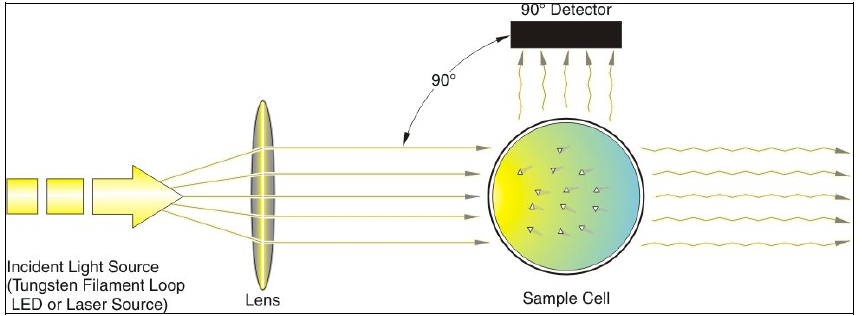
\includegraphics[scale=0.5]{figuras/sensorturbidez}
	\caption{Sensor para adquirir dados de temperatura.}
	\label{sensorturbidez}
\end{figure}
\FloatBarrier

A proposta do grupo é confeccionar o sensor, utilizando um LED infravermelho ou um diodo laser como emissor e um fotodiodo como receptor. Confeccionar também todo o circuito para o tratamento do sinal, como um amplificador de transimpedância, para que seja obtido um sinal de tensão. Além disso, calibrar o sensor para obtenção de medições confiáveis e precisas. A confecção deste sensor é viável e irá reduzir significantemente o custo do projeto.
Os maiores riscos previstos para a implementação deste dispositivo é a fabricação da ponta de prova que entrará em contato com a água, o posicionamento correto do emissor e do receptor e, por fim, a calibragem. 


Sensor de temperatura

O sensor de temperatura digital DS18B20 é capaz de medir em graus Celsius, com resolução de 9-bit a 12-bit (configurável) e possui uma função de alarme programável em memória não volátil para valores abaixo ou acima das temperaturas desejadas. A comunicação é feita por 1- fio, ou seja, precisa apenas de 1 pino do microcontrolador para transferir os dados. Pode operar entre -55ºC até +125ºC e com precisão de mais ou menos 0.5ºC se estiver operando dentro da faixa de -10ºC até +85ºC. Cada DS18B20 possui um número serial único de 64-bit, o que permite que vários DS18B20 funcionem no mesmo barramento 1- fio, permitindo conectar vários sensores em um microcontrolador.

É superior aos modelos DS1820 e DS18S20.

Características:

- Comunicação 1-fio, que necessita apenas de um pino do microcontrolador para fazer a linha de dados;
- Opera de 3V a 5.5V e pode ser alimentado pela linha de dados;
- Opera entre -55ºC até +125ºC, sendo a precisão de mais ou menos 0.5ºC se estiver operando dentro da faixa de -10ºC até +85ºC;
- resolução configurável pelo usuário de 9-bit à 12-bit;
- possui função de alarme programável;
- possui número de série único de 64-bit, o que permite ligar vários sensores no mesmo microcontrolador;

 \begin{figure} [!htp]
	\centering
	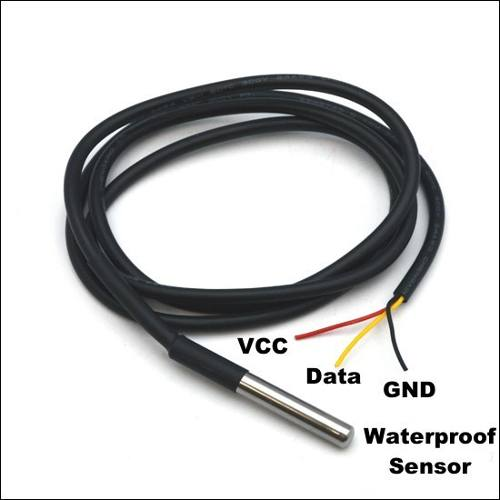
\includegraphics[scale=0.6]{figuras/sensortemp}
	\caption{Sensor para adquirir dados de temperatura.}
	\label{sensortemp}
\end{figure}
\FloatBarrier

Sensor de PH

O pH, medida do potencial Hidrogeniônico, determina o quão ácido ou alcalino é uma determinada solução. Uma solução neutra possui 7,0 de pH, enquanto uma solução ácida compreendida na faixa de pH menor que sete, porém, geralmente, próximas de 0. Uma solução com pH compreendida entre 7 e 14 é considerada alcalina. Por tratar-se de uma medida que varia numa escala logarítmica, toda unidade significa um aumento ou uma diminuição de 10 vezes. 

Uma solução alcalina, além de sua relação numérica com o pH, é capaz de neutralizar a acidez de uma solução. A alcalinidade de uma corrente de água é ampliada pela presença de hidróxidos (OH), carbonatos (CO3$^{2−}$) e bicarbonatos (HCO3$^{-}$), geralmente fornecido por pedras calcárias erodidas com o efeito da corrente de água. Águas extremamente alcalinas podem facilitar a dissolução de metais pesados, pois na medida em que os íons de hidrogênio tornam-se mais presentes na água, os cátions de metais com chumbo, alumínio, cobre e cádmio tendem a dissolver-se em água ou invés de depositar-se nos sedimentos no fundo. Este tipo de poluição afeta drasticamente a vida marinha e não própria para o consumo humano.

Uma solução ácida é, geralmente, associada com a presença de dióxido de carbônico dissolvido na água, provindo da atmosfera ou de matéria orgânica, seja por decomposição animal ou vegetal. A acidez extrema da água causa problemas de infraestrutura, corroendo canos e partes metálicas, causa também, desequilíbrio na vida marinha, visto que muitos peixes não toleram níveis elevados de acidez devido à adaptação ao ecossistema em que vivem. Acidez elevada pode ser danoso também para o ser humano, causando lesões na pele e olhos.

O pH é um importante indicador de qualidade da água, sendo a vida marinha a maior vítima de valores extremos. O nível ideal de pH da água está entre os valores de 6,5 a 9,0. A resolução 357/2005 do Conselho Nacional do Meio Ambiente (CONAMA) também estabelece um padrão aceitável de pH da água, este deve se compreender na faixa de 6,0 e 9,0 para águas doces.

O sensor para medir o pH é composto por dois eletrodos, um eletrodo de referência e outro eletrodo feito de vidro e preenchido com uma solução de pH fixo e valor 7,0. O potencial no eletrodo se mantém constante, ao passo que, o eletrodo de vidro será sensível à variação de pH. O potencial pode ser medido devido à troca de íons entre o eletrodo de vidro e a solução sendo medida. Sabendo-se o pH do eletrodo de vidro, sabe-se o pH da solução em questão.  A equação de Nernst fornece a força eletromotriz gerada por uma célula eletroquímica em função da concentração de íons nas soluções.

\begin{equation}
    E= E^{0} - \frac{RT}{nF} * ln(Q)
\end{equation}

Onde Q é o quociente da reação, E$^{0}$ é o potencial normal da célula, R é a constante universal dos gases, T é a temperatura em escala absoluta, F é a constante de Faraday, n é o número de mols de elétrons transferidos. Como a equação apresenta, a temperatura é um fator essencial para a medição do pH utilizando este tipo de sensor, assim o sensor de pH geralmente vem com um sensor de temperatura embutido.




\section{Subgrupo Estrutura}

\begin{figure} [!htp]
	\centering
	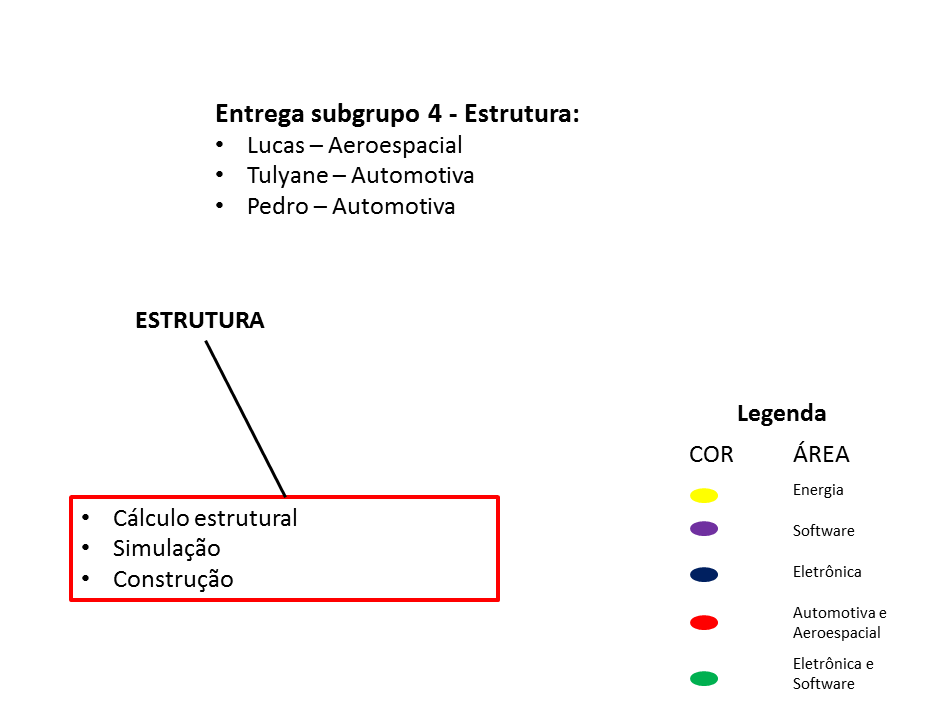
\includegraphics[scale=0.6]{figuras/subgrupoestrutura}
	\caption{Relaciona os membros e os problemas e os componentes que o subgrupo irá trabalhar na área de estrutura.}
	\label{subgrupoestrutura}
\end{figure}
\FloatBarrier

O veículo aquático de superfície em questão precisa ser caracterizado a fim de reunir as qualidades náuticas necessárias para sua missão. O seu projeto mecânico deve garantir a flutuabilidade, estabilidade, robustez, mobilidade e manobrabilidade do veículo. Desse modo há duas configurações possíveis que garantem as qualidades operacionais:

Embarcação de monocasco

Para essa configuração o casco do barco é convencional e disposto longitudinalmente. Nesse sentido, é necessário acoplar um motor na popa do barco que está em contato diretamente com a água. Além disso, um sistema de direcionamento, o leme, também precisa ser acoplado. A contrapartida dessa geometria, portanto, é em fazer a devida vedação entre motor, eixo e casco do barco. A necessidade energética também seria incrementada no caso da adoção do leme, pois sistemas eletromecânicos seriam necessários para seu funcionamento.

 \begin{figure} [!htp]
	\centering
	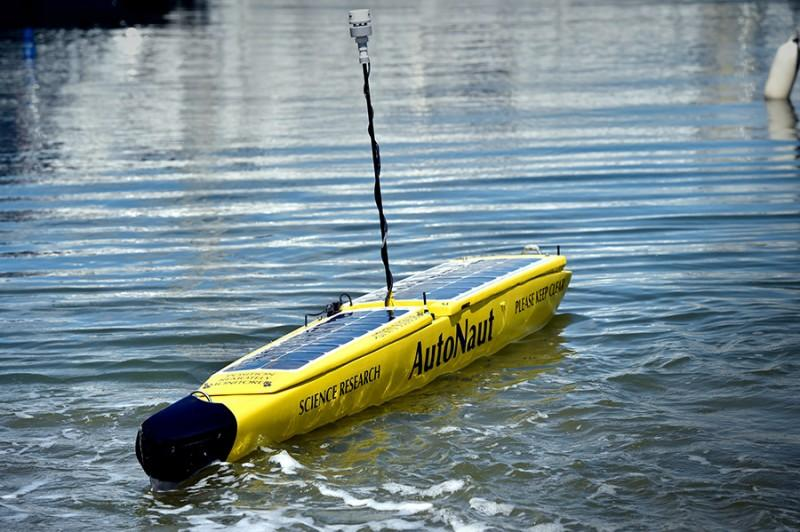
\includegraphics[scale=0.6]{figuras/monocasco}
	\caption{Ilustração de uma embarcação monocasco estilo caiaque.}
	\label{monocasco}
\end{figure}
\FloatBarrier


Embarcação catamarã (multi cascos)

De acordo com Marchaj (2000), um catamarã é um barco de propulsão à vela ou motor, com duas canoas paralelas idênticas (vulgarmente chamados “bananas”), presas por vigas, possibilitando montar uma plataforma ou cabine com os equipamentos necessários para a navegação. Devido a sua estrutura, comprimento relativo maior que a largura, os catamarãs podem navegar em alta velocidade com estabilidade relativamente boa, quando comparado com embarcações monocasco.
Esta configuração mostrou-se mais eficiente não apenas pelas qualidades náuticas apresentadas frente à configuração de monocasco, porém sua estrutura permite um arranjo mais eficiente de conjunto motor- transmissão, além de possibilitar um consumo energético mais econômico. 
O catamarã terá seus dois motores posicionados transversalmente ao seu casco, ou seja, um a estibordo e outro a bombordo. O controle de movimentos de guinada (yaw) será determinado pela diferença de velocidade angular das pás do sistema de propulsão. 
Esta configuração mostrou-se eficiente e suficiente para a missão e objetivo da embarcação.



- Materiais:


a) Fibra de vidro

A escolha do material para construção de uma determinada embarcação não é algo simples, visto que há uma variedade de opções para este fim, como o aço, o alumínio, a madeira, a fibra de vidro, ou a combinação destes. O custo e disponibilidade da matéria-prima são alguns dos principais fatores que influenciam na escolha do material.

A fibra de vidro revestida com uma resina é uma das opções mais populares para a construção de barcos não apenas pelo seu preço, mas pela sua durabilidade. Uma das principais vantagens da fibra sobre a madeira, alumínio ou aço, é a variedade de estruturas que se pode conseguir utilizando outros materiais. As propriedades químicas e mecânicas da fibra de vidro dão ao construtor a liberdade para adaptar o seu projeto e fazer melhorias à necessidade de cada peça e ao processo de fabricação.

De acordo com Nasseh (2011, p. 66), dentre os tipos de vidro, designados pelas letras do alfabeto, o vidro tipo E é geralmente o mais utilizado devido ao seu caráter de isolamento térmico, baixo teor alcalino, boa resistência à tração, boa rigidez em relação á flexão e pelo seu custo, e é, sem dúvida, o mais popular entre os construtores de barcos em todo o mundo. 


b) Resina Epóxi

O polímero (poly + meros) é um tipo de material composto por macromoléculas, que, por sua vez, são compostas pela repetição do mero. Portanto, poly (muitos) e meros (partes) dão alusão ao material que é formado pela reação em cadeia entre os monômeros (CALLISTER, 2002).

Na construção de embarcações, a resina tem como principal função prender as fibras na posição planejada, além de proteger o material contra agressões externas, corrosão e outros problemas ocasionados pelo contato com a água. A resina tem uma resistência inferior à das fibras, assim, objetos fabricados a partir de resina são fracos, mas se utilizado com fibras de alta resistência tornam o material viável para diversas aplicações na Engenharia, devido as propriedades mecânicas adquiridas nessa combinação. 

Na construção de barcos, as resinas mais utilizadas são do tipo poliéster, estervinílicas e epóxi, conhecidas como termofixas, ou seja, são insolúveis após serem catalisadas e curadas, não sendo possível a reutilização para outras aplicações, diferentemente das resinas termoplásticas. 


A escolha da resina não se restringe apenas ao preço, mas ao seu custo-benefício, visto que a construção de um barco não é algo feito em grande escala, como na Automotiva, permitindo ao construtor uma liberdade de escolha de material que melhor se adeque ao seu projeto, processo de fabricação e orçamento.

As resinas epóxi são termorrígidas de alto desempenho e são matérias-primas em vários setores industriais, sendo muito utilizadas pelos construtores pelas suas excelentes qualidades mecânicas, boa adesão a outros materiais, como metal e madeira, e uma boa estabilidade química. Entre suas aplicações estão recobrimentos protetivos, adesivos e compósitos estruturais.

Tabela de propriedades típicas de resina epóxi e fibra de vidro. (Fonte: Adaptado  - Callister, 2012




\begin{table}[h]
	\centering
	\label{compaco}	
	\begin{tabular}{cccc}
		\toprule
		\textbf{ } & \textbf{M.Epoxi  + F. vidro(60\%)} & \textbf{F.vidroE}& \textbf{ResinaEpóxi} \\
		\midrule
Densidade Relativa&2,1&2,58&1,25\\
Módulo de tração–Long.&45 GPa&-&-\\
Módulo de tração–Trans.&1020 MPa&-&-\\
Limite a tração–Longitudinal&40 MPa&3,45GPa&-\\
Limite a tração–Trans.&-&-&-\\
Módulo de elasticidade&-&72,5GPa&2,4GPa\\
Massa específica&-&2,58g/$cm^{3}$ &1,14g/$cm^{3}$\\
		\bottomrule
	\end{tabular}	
	\caption{Tabela de propriedades típicas de resina epóxi e fibra de vidro. (Fonte: Adaptado  - Callister, 2012}
\end{table}


c) Alumínio 

As características físico-químicas do alumínio fazem dele um dos metais mais utilizados na indústria atual, isso se deve pelo seu baixo peso específico, ou seja, sua leveza, aliada à sua resistência a corrosão. 

O alumínio é um material de fácil transformação, aceitando qualquer tipo de processo metalúrgico e pode ser combinado com a maioria dos metais de engenharia, os chamados elementos de liga, em que a partir dessas combinações se obtém características desejáveis ao seu produto, como por exemplo o limite de resistência à tração do aço tem seu valor aumentado em função da liga, do trabalho a frio e do tratamento térmico dado a ele. 






\begin{table}[h]
	\centering
	\label{compaco}	
	\begin{tabular}{ccc}
		\toprule
		\textbf{Propriedades físicas típicas} & \textbf{Alumínio} & \textbf{Aço} \\
		\midrule
Densidade (g/$cm^3$) & 2,70 & 7,86 \\
Temperatura de fusão (ºC) & 660 & 1500 \\
Módulo de elasticidade (Mpa) & 70000 & 2050000 \\
Coeficiente de dilatação térmica (L/ºC)& 23 * 10$^{-6}$ & 11,7 * 10$^{-6}$ \\
Condutibilidade térmica a 25ºC (cal/cm/ºC) & 0,53 & 0,12 \\
Condutibilidade elétrica (\% IACS) & 61 & 14,5 \\
		\bottomrule
	\end{tabular}	
	\caption{Comparação entre as propriedades físicas alumínio e aço}
\end{table}

Elementos complementares do projeto

a) Eixo

Para transmissão de movimento de rotação e torque de um 
ponto ao outro é usado um eixo de transmissão acoplado a uma máquina rotativa. O eixo pode ser uma parte integrante da máquina rotativa ou um eixo livre conectado a máquina por meio de um acoplamento. Eixos de transmissão de rotação estão submetidos a cargas de flexão e torção; torção devido ao torque transmitido e flexão devido às carregamentos transversais. Geralmente um eixo de transmissão possui secção transversal circular. Devido aos esforços submetidos sobre o eixo, o aço é o material mais utilizado para confecção do mesmo, pois possui um elevado módulo de elasticidade, atribuindo uma maior confiabilidade ao elemento. 

b) Engrenagens

Engrenagens são usadas para transmitir torque e velocidade angular em uma ampla variedade de aplicações (NORTON, 2004). A transmissão de movimento tem normalmente como finalidade aproveitar o máximo de potência gerada em trabalho mecânico útil. O movimento de rotação entre as engrenagens ocorre por meio do contato de seus dentes.

Os materiais mais usados na fabricação de engrenagens são: aço-liga-fundido, ferro fundido, cromo níquel, alumínio, bronze fosforoso, náilon (FRANCESCHI; ANTONELLO).
A engrenagem cilíndrica é a do tipo mais simples, opera com eixos paralelos e tem dentes paralelos ao eixo de coordenadas do eixo. Esse tipo de engrenagem que será utilizada no projeto.

c) Parafusos e fixadores

A determinação e o uso de elementos fixadores adequados presentes em um projeto é primordial para o sucesso do mesmo. Para manter peças mecânicas unidas, são usados parafusos, pinos, grampos, etc. Que devem resistir à carga de tração e de cisalhamento.

d) Elementos de vedação

Vedação é o processo empregado para impedir a passagem, de maneira estática ou dinâmica, de líquidos, gases e sólidos particulados de um meio para outro. São elementos destinados a impedir a saída de líquidos e gases, assim como da entrada de sujeira ou pó em máquinas e equipamentos (FRANCESCHI; ANTONELLO).

Ferramentas para execução do projeto


Para a construção do barco autônomo, será necessária a utilização de algumas ferramentas e maquinários. Segue abaixo uma lista das principais ferramentas.

\begin{itemize}
  \item      Equipamento de proteção individual (EPI)
\item         Furadeira            
\item        Lixadeira
\item      Cortador de isopor, estilete
\item        Instrumentos de medidas
\item       Fixadores
\item        Chaves
\item        Alicates
\item        Torno
\item       Fresadora
\item        Serra fita
\end{itemize}


Descrição da estrutura do produto

Tendo como base as informações levantadas anteriormente, o barco autônomo (RoBoatT) será construído com as características de um trimarã (embarcação composta por três cascos), esse tipo de embarcação possui estabilidade lateral maior quando comparado a um monocasco, e alta capacidade de manobra.

A propulsão será realizada por dois motores, acoplados ao casco principal, sendo que as hélices estarão dispostas lateralmente ao casco principal. Por não encontrarmos um motor convencional para barcos que atendesse o nosso projeto, foi necessário essa idealização de dois motores e as hélices dispostas lateralmente. O barco não irá possuir leme, para conseguir manobrá-lo, os motores serão controlados eletronicamente para que a diferença de velocidades entres eles faça com que o barco consiga realizar manobras. 

Atrás do casco principal terá uma estrutura para acoplar os componentes eletrônicos que vão fazer as medições diretamente na água. Dentro do casco principal terá alguns componentes eletrônicos que não podem entrar em contato com água, além dos motores, por este motivo, é necessário uma boa vedação por onde vão passar os eixos e uma tampa de cobertura dos casco, porém uma parte precisa estar aberta para facilitar o envio/recebimento dos dados.

O material utilizado para construção dos cascos será um composto de isopor reforçado com fibra de vidro. Com este composto é possível construir uma embarcação com boa flutuabilidade e resistência, além do baixo peso. Os eixos serão feitos de aço 1020, por causa do seu elevado módulo de elasticidade, a fim de se minimizar as deflexões. Para conectar o casco principal aos cascos laterais, será usado cano PVC. 

 \begin{figure} [!htp]
	\centering
	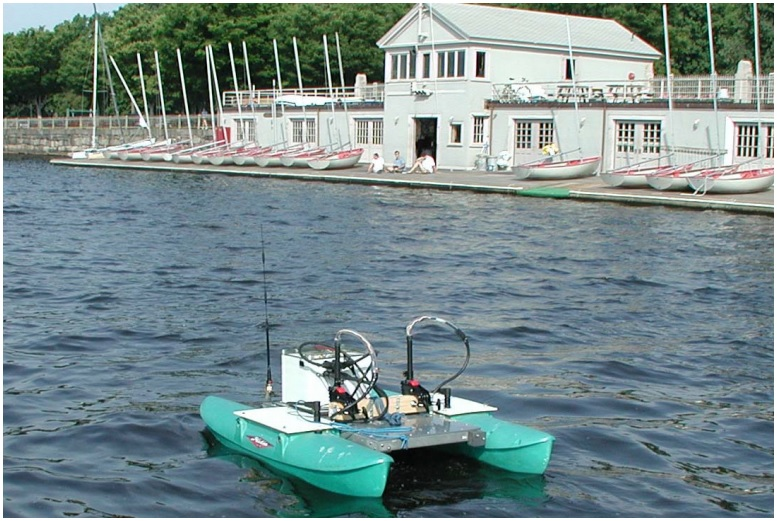
\includegraphics[scale=0.7]{figuras/catamara}
	\caption{Figura ilustrativa catamarã.}
	\label{catamara}
\end{figure}
\FloatBarrier

Desenhos técnicos de planejamento da estrutura



\FloatBarrier
 \begin{figure} [!htp]
	\centering
	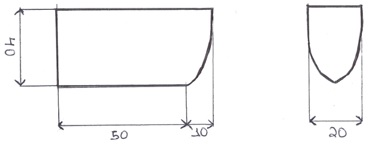
\includegraphics[scale=1]{figuras/roboat_cascolateral}
	\caption{Desenho técnico vista casco lateral.}
	\label{dtcl}
\end{figure}
\FloatBarrier



\FloatBarrier
 \begin{figure} [!htp]
	\centering
	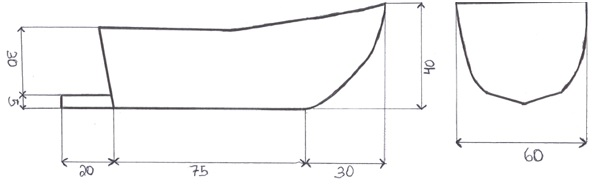
\includegraphics[scale=1]{figuras/roboat_lateral}
	\caption{Desenho técnico vista lateral.}
	\label{dtl}
\end{figure}
\FloatBarrier

\FloatBarrier
 \begin{figure} [!htp]
	\centering
	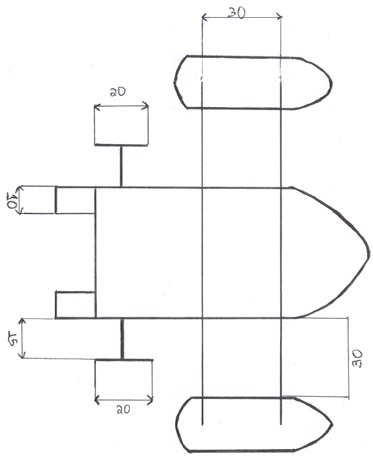
\includegraphics[scale=1]{figuras/roboat_sup}
	\caption{Desenho técnico vista superior.}
	\label{dts}
\end{figure}
\FloatBarrier


\section{Subgrupo software de controle e comunicação}

\subsection{Funcionalidades}

\begin{itemize}
    \item Foram identificadas as seguintes funcionalidades:
    \item Cadastrar usuário no sistema;
    \item Logar usuário no sistema;
    \item Editar perfil do usuário;
    \item Excluir usuário do sistema;
    \item Mostrar mapa local e localização do barco;
    \item Determinar pontos de coleta no mapa;
    \item Controlar o barco manualmente;
    \item Realizar coleta de água;
    \item Realizar coleta de dados;
    \item Manter coleta no sistema;
    \item Gerenciar histórico de coletas;
    \item Navegar de forma autônoma;
    \item Gerar relatório das coletas.
\end{itemize}

\subsection{Protótipos}

No desenvolvimento de software a utilização de protótipos é efetiva para entender os requisitos, diminuir a complexidade do  problema  e  prover  maneiras   de  validação  do  design  do  sistema  no  início  do projeto.  A  etapa  de  se  realizar  o  protótipo  se  resume  em  produzir versões    com o intuito de  apresentar    diversos    aspectos    deste (BERNSTEIN, 1996).

Um  protótipo  pode  representar  o  produto  final,  porém  pode  também  ser completamente  descartável,  o  protótipo  é  apenas  um  exemplo  de  como  o software final pode ser, mas não necessariamente como será (BERNSTEIN, 1996).

Protótipos são úteis para (BERNSTEIN, 1996):

\begin{enumerate}
    \item Demonstrar  o  que  é  possível  fazer,  de  acordo  com  a  tecnologia adotada;
    \item Demonstrar uma ideia de como o aspecto visual do software será;
    \item Iteração com o cliente;
    \item Permitir novas ideias para o produto final;
    \item Uma maneira de validar e evoluir os requisitos do sistema.
\end{enumerate}

Requisitos Funcionais


Para se desenvolver um software a utilização de protótipos auxilia no levantamento dos requisitos e diminui o risco de uma manutenção árdua nas funcionalidades e na interface do produto. Modificar as versões do protótipo é mais eficiente que modificar o sistema.

Um  protótipo  pode  representar  o  produto  final,  porém  pode  também  ser
completamente  descartável,  o  protótipo  é  apenas  um  exemplo  de  como  o  software
final pode ser, mas não necessariamente como será (BERNSTEIN, 1996).

Protótipos são úteis para melhorar a interação com o cliente, permitir novas ideias para o produto final, demonstrar a possibilidade de se fazer o sistema com a tecnologia adotada,  permitir a validação e a evolução do sistema.
A  ferramenta  utilizada  para  criação  dos  protótipos  foi  a piktochart versão livre. 
O  prototipo  inicial  consiste  de  5  páginas:  página  inicial, página de monitoramento, página de controle, página de relatórios a página de geração de gráficos. Estas telas tem como objetivo visualizar controlar o roboat e visualizar os dados coletados por este.
Na tela inicial do sistema, o usuário pode escolher o que deseja fazer. Ele poderá monitorar, controlar ou ver os dados coletados pelo roboat.

 \begin{figure} [!htp]
	\centering
	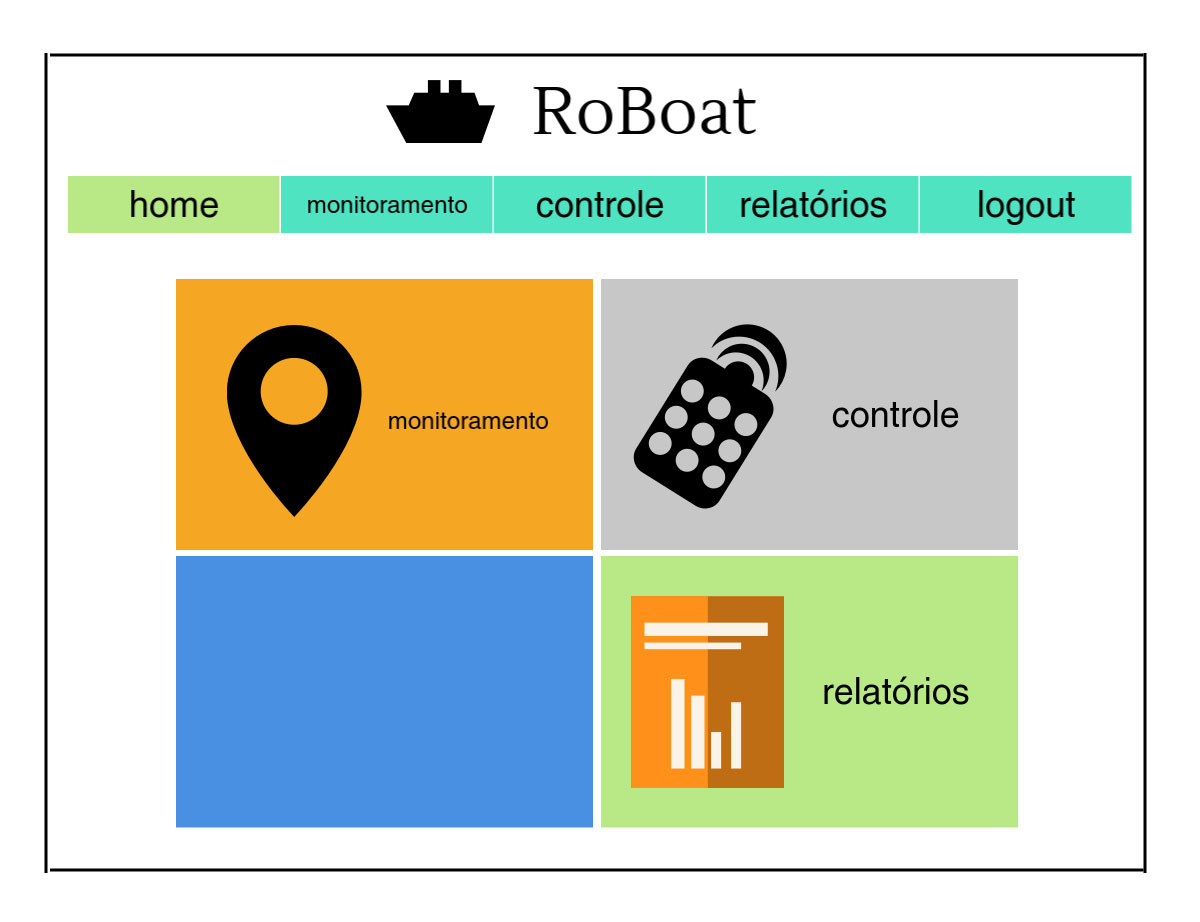
\includegraphics[scale=0.3]{figuras/prototipo-6}
	\caption{Prototipo 6}
	\label{Prototipo 6}
\end{figure}
\FloatBarrier

Na tela subsequente, pode-se verificar como será visualizada, pelo usuário, a página de monitoramento do roboat. Esta tela mostrará a localização do barco em um mapa do lado direito, e do lado esquerdo mostrará suas latitude, longitude e porcentagem da bateria. Por fim o usuário poderá inserir manualmente os 3 pontos que o barco deverá coletar a água e enviar os dados referente à coleta.


\FloatBarrier
 \begin{figure} [!htp]
	\centering
	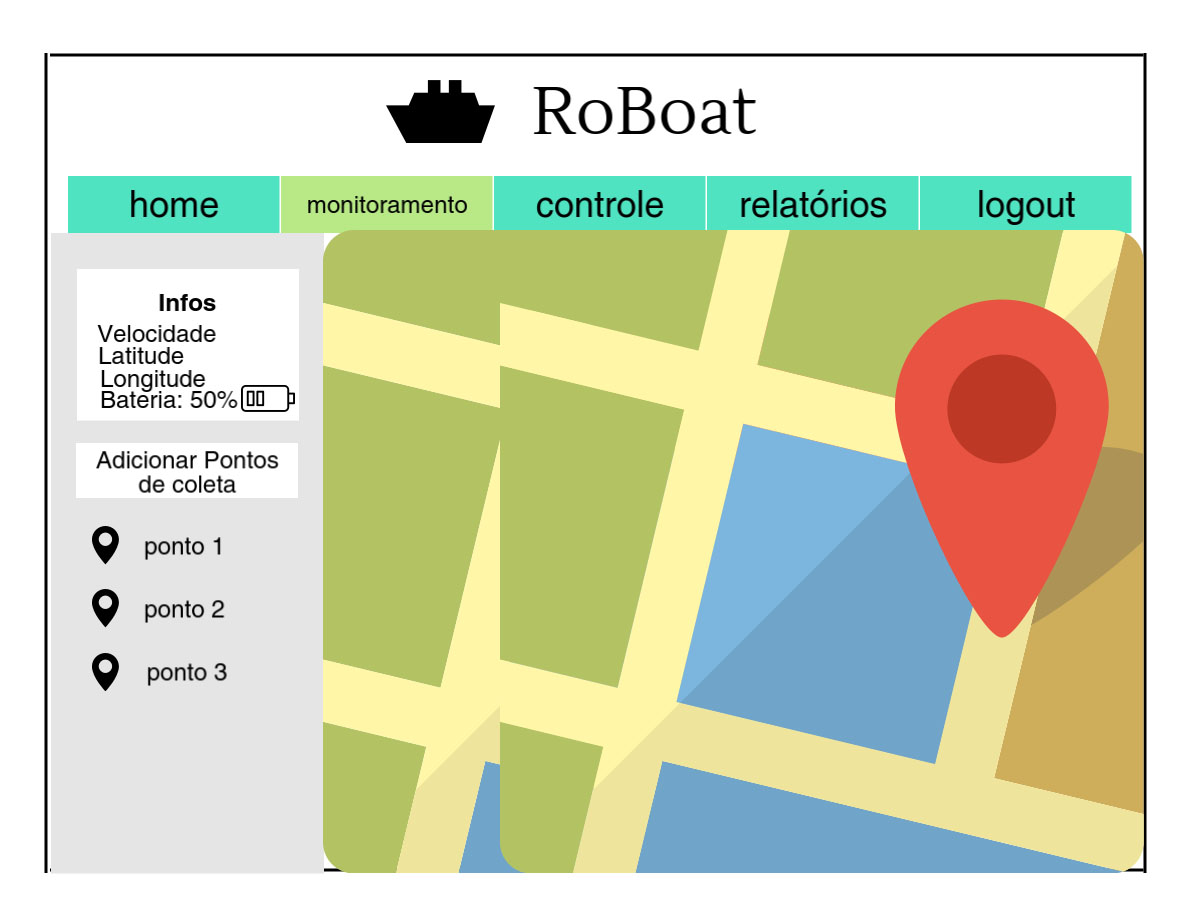
\includegraphics[scale=0.3]{figuras/prototipo-5}
	\caption{prototipo 5}
	\label{fig:prototipo5}
\end{figure}
\FloatBarrier

Na tela de controle, o usuário poderá controlar o barco pelas setas do computador ou pelas setas mostradas na página. Após concluir-se o controle do barco o usuário poderá clicar no botão "coletar” e o RoBoat coletará e enviará os dados referentes à coleta.

 \begin{figure} [!htp]
	\centering
	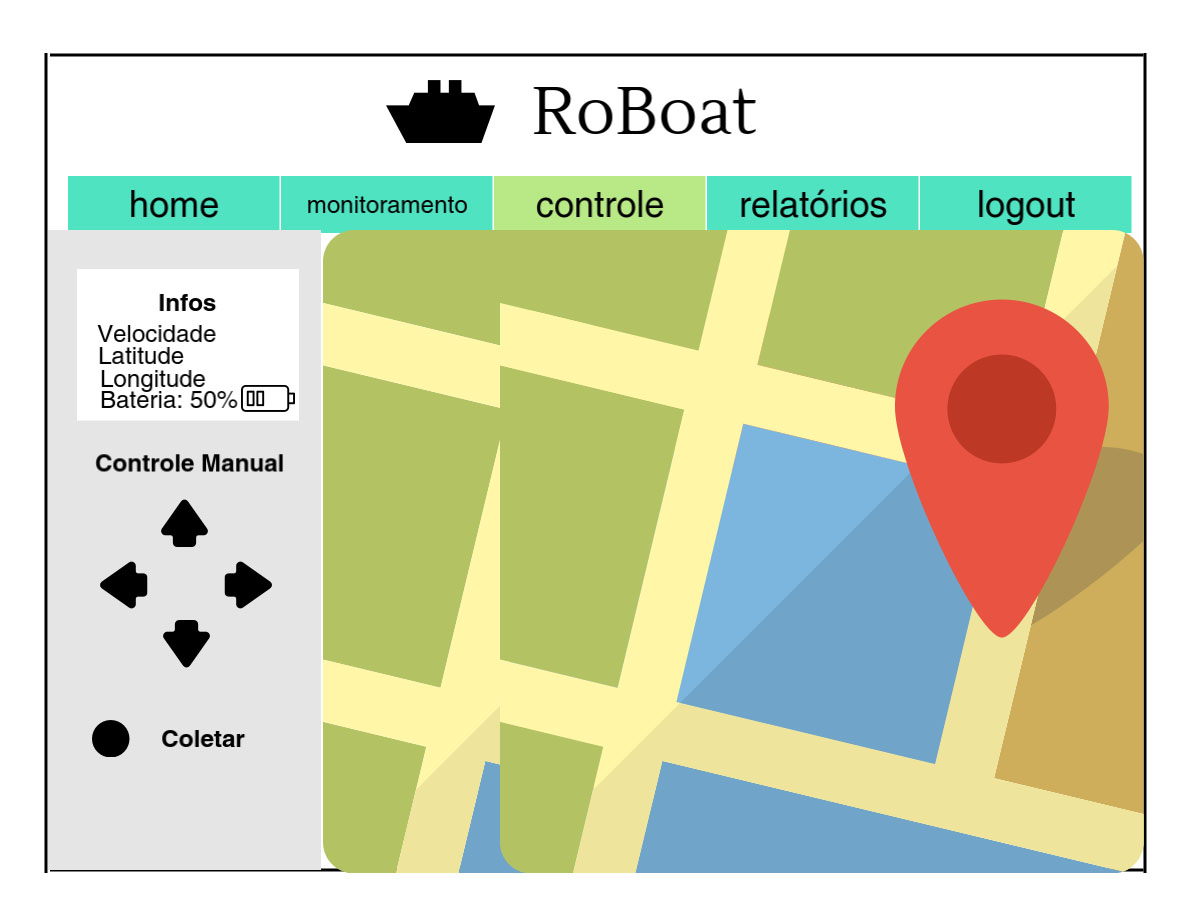
\includegraphics[scale=0.3]{figuras/prototipo-4}
	\caption{prototipo4}
	\label{Prototipo 4}
\end{figure}
\FloatBarrier

 \begin{figure} [!htp]
	\centering
	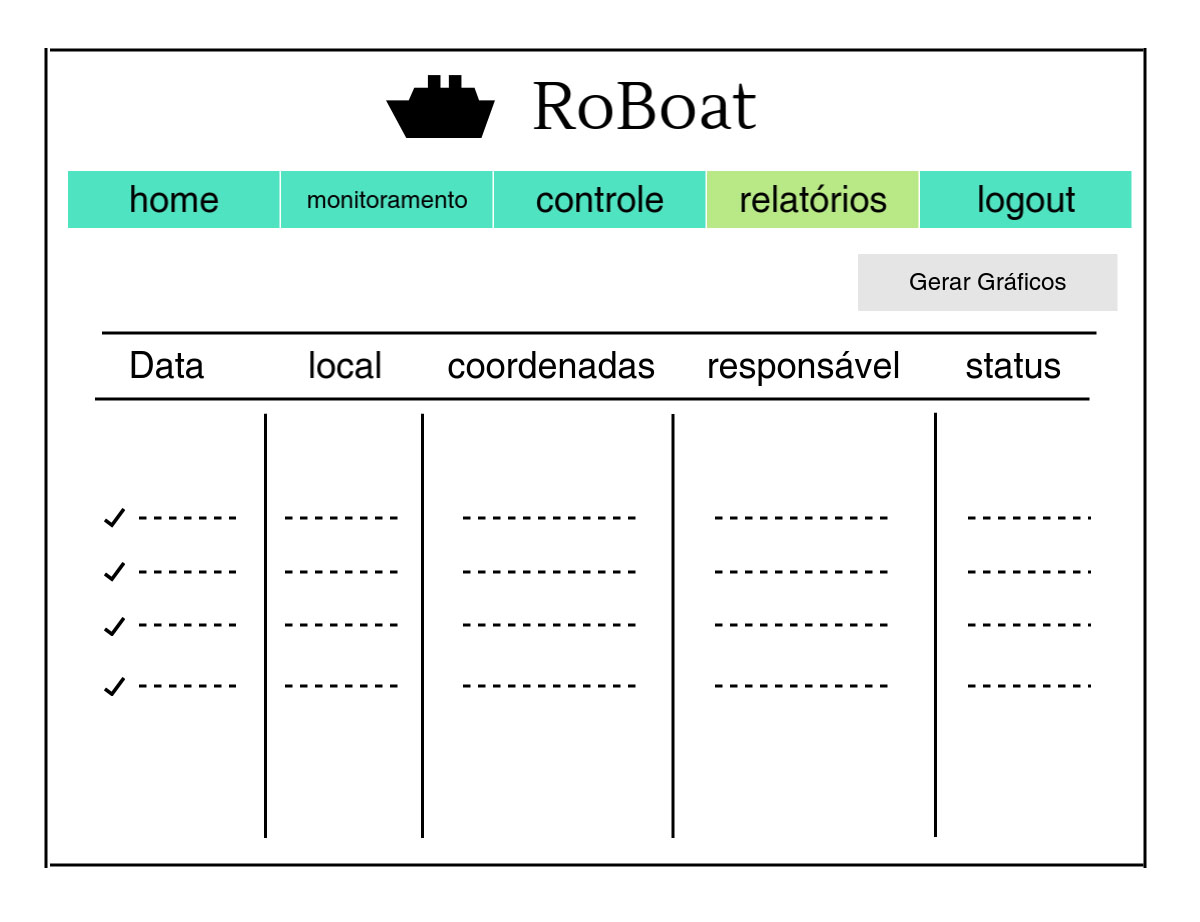
\includegraphics[scale=0.3]{figuras/prototipo-3}
	\caption{prototipo3}
	\label{Prototipo 3}
\end{figure}
\FloatBarrier

Na tela referente aos relatórios, o usuário poderá verificar a data, o local, as coordenadas, o responsável e o status das ultimas coletas. Após ver esses dados o usuário poderá selecionar algumas dessas coletas e gerar um gráfico para compará-las.Na tela dos gráficos os dados serão apresentados para o usuário e ele poderá analisar os gráficos , que serão apresentatados em forma de barras.

 \begin{figure} [!htp]
	\centering
	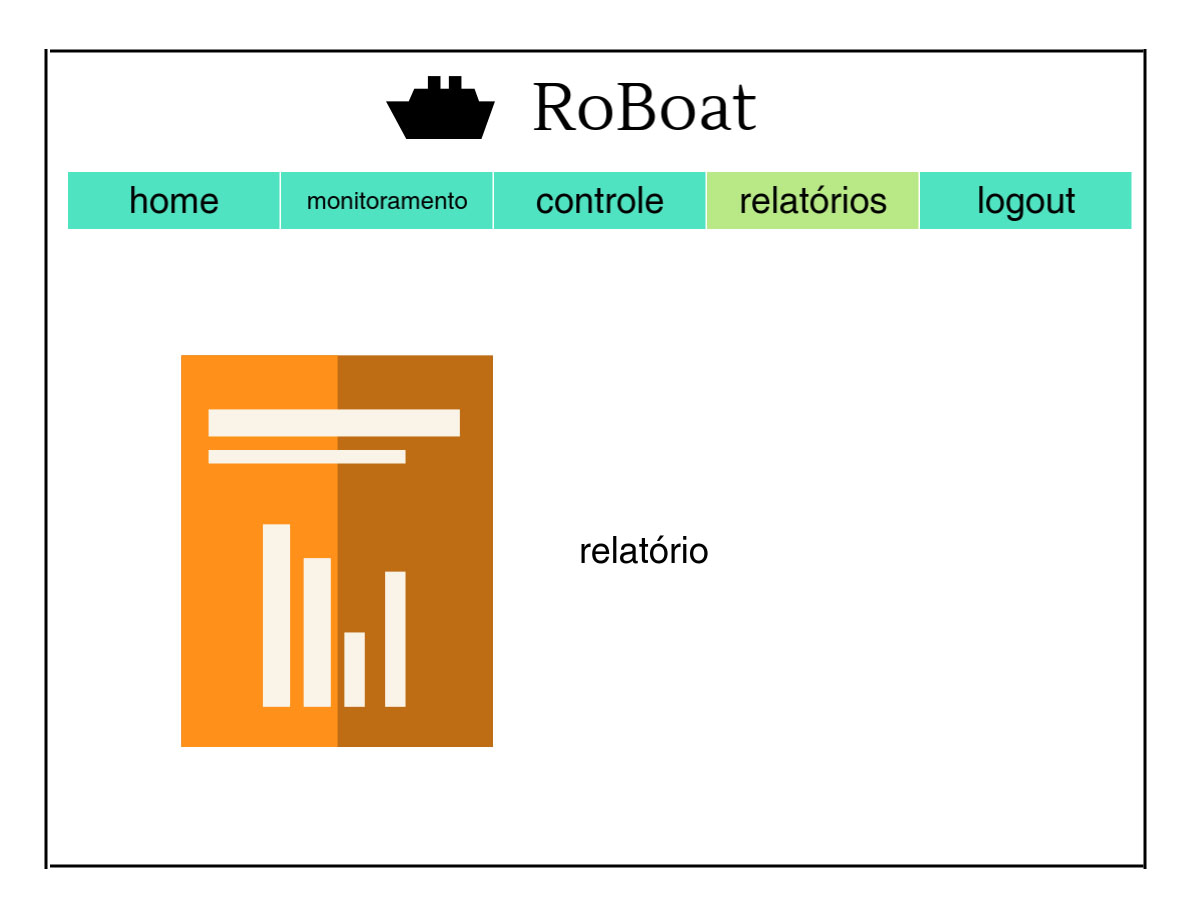
\includegraphics[scale=0.3]{figuras/prototipo-2}
	\caption{prototipo1}
	\label{Prototipo 2}
\end{figure}
\FloatBarrier

Estas são as páginas que mostram os requisitos levantados até este momento. Vale salientar que no processo de desenvolvimento de software os requisitos são voláteis e podem mudar de acordo com o tempo. Fazendo com que o protótipo possa mudar ou até mesmo ser descartado.

\subsection{Arquitetura do Software}


A arquitetura de software é a estrutura do sistema, a qual é composta de elementos de software, das propriedades externamente visíveis desses elementos, e dos relacionamentos entre eles; é a abstração do sistema (Bass, 2003).

Model-view-controller (MVC) é um padrão de arquitetura de software. Com o aumento da complexidade das aplicações desenvolvidas torna-se fundamental a separação entre os dados (Model) e o layout (View). Desta forma, alterações feitas no layout não afetam a manipulação de dados, e estes poderão ser reorganizados sem alterar o layout. 

Como o software que controlará e se comunicará com o Roboat será construído na linguagem Ruby com o framework Rails, ao qual utiliza a o padrão de arquitetura MVC, essa é arquitetura adotada.

Neste modelo, a aplicação é dividida em três partes:

\begin{itemize}
    \item Modelo (MODEL): Lógica de negócio, representa as regras para manipulação dos dados e no Rails são usadas para gerenciar as regras de interação com as tabelas do banco de dados.

    \item Visão (VIEW): Camada de interface com o usuário. Nesta camada o usuário vê o estado do modelo e pode manipular a interface, para ativar a lógica do negócio;

    \item Controlador (CONTROLLER): Conectam a modelo (model) a visão (view) e transforma eventos gerados pela interface em ações de negócio, alterando o modelo. Assim, são responsáveis pelo processamento das requisições recebidas pelo navegador, indo até as modelos para acessar os dados e posteriormente passando esses dados para a interface gráfica, a view.
\end{itemize}

caso-de-uso.png

 \begin{figure} [!htp]
	\centering
	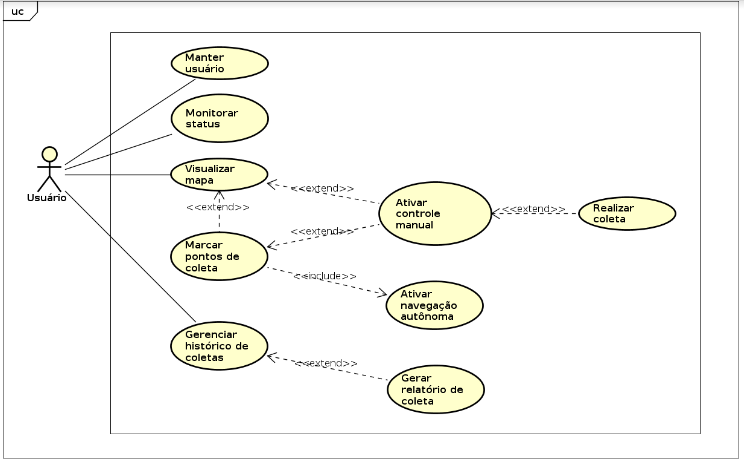
\includegraphics[scale=0.6]{figuras/caso-de-uso.png}
	\caption{Diagrama de Caso de Uso}
	\label{fig:caso-de-uso}
\end{figure}
\FloatBarrier

\textbf{UC1 - Manter Usuário}

	Caso de uso cujo o objetivo é realizar cadastro de usuários, editar cadastro, visualizar lista de cadastros e excluir cadastro do sistema.

\textbf{UC2 - Monitorar status}

	Caso de uso cujo o objetivo é mostrar para o usuário dados como velocidade, localização (latitude e longitude) e status da bateria do RoBoat.

\textbf{UC4 - Visualizar Mapa}

	Caso de uso cujo o objetivo é mostrar o mapa local e mostrar a localização do RoBoat.

\textbf{UC5 - Marcar pontos de coleta}

	Caso de uso cujo o objetivo é determinar os pontos  de coleta.
	
\textbf{UC6 - Controlar barco manualmente}

	Caso de uso cujo objetivo é disponibilizar para o usuário o total controle direcional do RoBoat.

\textbf{UC7 - Ativar navegação autônoma}

	Caso de uso cujo o objetivo é colocar o RoBoat em modo autônomo de navegação e coleta de dados.

\textbf{UC8 - Realizar coleta}

	Caso de uso cujo o objetivo é enviar o comando para o RoBoat realizar a coleta de água e de dados da água.

\textbf{UC9 - Gerar gráfico}

	Caso de uso cujo o objetivo é gerar gráfico dos parâmetros de análise da água.

\textbf{UC10 - Gerenciar histórico de coletas}

	Caso de uso cujo o objetivo é mostrar para o usuário a lista de coletas já realizadas.
	
